
% Default to the notebook output style

    


% Inherit from the specified cell style.




    
\documentclass[11pt]{article}

    
    
    \usepackage[T1]{fontenc}
    % Nicer default font (+ math font) than Computer Modern for most use cases
    \usepackage{mathpazo}

    % Basic figure setup, for now with no caption control since it's done
    % automatically by Pandoc (which extracts ![](path) syntax from Markdown).
    \usepackage{graphicx}
    % We will generate all images so they have a width \maxwidth. This means
    % that they will get their normal width if they fit onto the page, but
    % are scaled down if they would overflow the margins.
    \makeatletter
    \def\maxwidth{\ifdim\Gin@nat@width>\linewidth\linewidth
    \else\Gin@nat@width\fi}
    \makeatother
    \let\Oldincludegraphics\includegraphics
    % Set max figure width to be 80% of text width, for now hardcoded.
    \renewcommand{\includegraphics}[1]{\Oldincludegraphics[width=.8\maxwidth]{#1}}
    % Ensure that by default, figures have no caption (until we provide a
    % proper Figure object with a Caption API and a way to capture that
    % in the conversion process - todo).
    \usepackage{caption}
    \DeclareCaptionLabelFormat{nolabel}{}
    \captionsetup{labelformat=nolabel}

    \usepackage{adjustbox} % Used to constrain images to a maximum size 
    \usepackage{xcolor} % Allow colors to be defined
    \usepackage{enumerate} % Needed for markdown enumerations to work
    \usepackage{geometry} % Used to adjust the document margins
    \usepackage{amsmath} % Equations
    \usepackage{amssymb} % Equations
    \usepackage{textcomp} % defines textquotesingle
    % Hack from http://tex.stackexchange.com/a/47451/13684:
    \AtBeginDocument{%
        \def\PYZsq{\textquotesingle}% Upright quotes in Pygmentized code
    }
    \usepackage{upquote} % Upright quotes for verbatim code
    \usepackage{eurosym} % defines \euro
    \usepackage[mathletters]{ucs} % Extended unicode (utf-8) support
    \usepackage[utf8x]{inputenc} % Allow utf-8 characters in the tex document
    \usepackage{fancyvrb} % verbatim replacement that allows latex
    \usepackage{grffile} % extends the file name processing of package graphics 
                         % to support a larger range 
    % The hyperref package gives us a pdf with properly built
    % internal navigation ('pdf bookmarks' for the table of contents,
    % internal cross-reference links, web links for URLs, etc.)
    \usepackage{hyperref}
    \usepackage{longtable} % longtable support required by pandoc >1.10
    \usepackage{booktabs}  % table support for pandoc > 1.12.2
    \usepackage[inline]{enumitem} % IRkernel/repr support (it uses the enumerate* environment)
    \usepackage[normalem]{ulem} % ulem is needed to support strikethroughs (\sout)
                                % normalem makes italics be italics, not underlines
    

    
    
    % Colors for the hyperref package
    \definecolor{urlcolor}{rgb}{0,.145,.698}
    \definecolor{linkcolor}{rgb}{.71,0.21,0.01}
    \definecolor{citecolor}{rgb}{.12,.54,.11}

    % ANSI colors
    \definecolor{ansi-black}{HTML}{3E424D}
    \definecolor{ansi-black-intense}{HTML}{282C36}
    \definecolor{ansi-red}{HTML}{E75C58}
    \definecolor{ansi-red-intense}{HTML}{B22B31}
    \definecolor{ansi-green}{HTML}{00A250}
    \definecolor{ansi-green-intense}{HTML}{007427}
    \definecolor{ansi-yellow}{HTML}{DDB62B}
    \definecolor{ansi-yellow-intense}{HTML}{B27D12}
    \definecolor{ansi-blue}{HTML}{208FFB}
    \definecolor{ansi-blue-intense}{HTML}{0065CA}
    \definecolor{ansi-magenta}{HTML}{D160C4}
    \definecolor{ansi-magenta-intense}{HTML}{A03196}
    \definecolor{ansi-cyan}{HTML}{60C6C8}
    \definecolor{ansi-cyan-intense}{HTML}{258F8F}
    \definecolor{ansi-white}{HTML}{C5C1B4}
    \definecolor{ansi-white-intense}{HTML}{A1A6B2}

    % commands and environments needed by pandoc snippets
    % extracted from the output of `pandoc -s`
    \providecommand{\tightlist}{%
      \setlength{\itemsep}{0pt}\setlength{\parskip}{0pt}}
    \DefineVerbatimEnvironment{Highlighting}{Verbatim}{commandchars=\\\{\}}
    % Add ',fontsize=\small' for more characters per line
    \newenvironment{Shaded}{}{}
    \newcommand{\KeywordTok}[1]{\textcolor[rgb]{0.00,0.44,0.13}{\textbf{{#1}}}}
    \newcommand{\DataTypeTok}[1]{\textcolor[rgb]{0.56,0.13,0.00}{{#1}}}
    \newcommand{\DecValTok}[1]{\textcolor[rgb]{0.25,0.63,0.44}{{#1}}}
    \newcommand{\BaseNTok}[1]{\textcolor[rgb]{0.25,0.63,0.44}{{#1}}}
    \newcommand{\FloatTok}[1]{\textcolor[rgb]{0.25,0.63,0.44}{{#1}}}
    \newcommand{\CharTok}[1]{\textcolor[rgb]{0.25,0.44,0.63}{{#1}}}
    \newcommand{\StringTok}[1]{\textcolor[rgb]{0.25,0.44,0.63}{{#1}}}
    \newcommand{\CommentTok}[1]{\textcolor[rgb]{0.38,0.63,0.69}{\textit{{#1}}}}
    \newcommand{\OtherTok}[1]{\textcolor[rgb]{0.00,0.44,0.13}{{#1}}}
    \newcommand{\AlertTok}[1]{\textcolor[rgb]{1.00,0.00,0.00}{\textbf{{#1}}}}
    \newcommand{\FunctionTok}[1]{\textcolor[rgb]{0.02,0.16,0.49}{{#1}}}
    \newcommand{\RegionMarkerTok}[1]{{#1}}
    \newcommand{\ErrorTok}[1]{\textcolor[rgb]{1.00,0.00,0.00}{\textbf{{#1}}}}
    \newcommand{\NormalTok}[1]{{#1}}
    
    % Additional commands for more recent versions of Pandoc
    \newcommand{\ConstantTok}[1]{\textcolor[rgb]{0.53,0.00,0.00}{{#1}}}
    \newcommand{\SpecialCharTok}[1]{\textcolor[rgb]{0.25,0.44,0.63}{{#1}}}
    \newcommand{\VerbatimStringTok}[1]{\textcolor[rgb]{0.25,0.44,0.63}{{#1}}}
    \newcommand{\SpecialStringTok}[1]{\textcolor[rgb]{0.73,0.40,0.53}{{#1}}}
    \newcommand{\ImportTok}[1]{{#1}}
    \newcommand{\DocumentationTok}[1]{\textcolor[rgb]{0.73,0.13,0.13}{\textit{{#1}}}}
    \newcommand{\AnnotationTok}[1]{\textcolor[rgb]{0.38,0.63,0.69}{\textbf{\textit{{#1}}}}}
    \newcommand{\CommentVarTok}[1]{\textcolor[rgb]{0.38,0.63,0.69}{\textbf{\textit{{#1}}}}}
    \newcommand{\VariableTok}[1]{\textcolor[rgb]{0.10,0.09,0.49}{{#1}}}
    \newcommand{\ControlFlowTok}[1]{\textcolor[rgb]{0.00,0.44,0.13}{\textbf{{#1}}}}
    \newcommand{\OperatorTok}[1]{\textcolor[rgb]{0.40,0.40,0.40}{{#1}}}
    \newcommand{\BuiltInTok}[1]{{#1}}
    \newcommand{\ExtensionTok}[1]{{#1}}
    \newcommand{\PreprocessorTok}[1]{\textcolor[rgb]{0.74,0.48,0.00}{{#1}}}
    \newcommand{\AttributeTok}[1]{\textcolor[rgb]{0.49,0.56,0.16}{{#1}}}
    \newcommand{\InformationTok}[1]{\textcolor[rgb]{0.38,0.63,0.69}{\textbf{\textit{{#1}}}}}
    \newcommand{\WarningTok}[1]{\textcolor[rgb]{0.38,0.63,0.69}{\textbf{\textit{{#1}}}}}
    
    
    % Define a nice break command that doesn't care if a line doesn't already
    % exist.
    \def\br{\hspace*{\fill} \\* }
    % Math Jax compatability definitions
    \def\gt{>}
    \def\lt{<}
    % Document parameters
    \title{proj2}
    
    
    

    % Pygments definitions
    
\makeatletter
\def\PY@reset{\let\PY@it=\relax \let\PY@bf=\relax%
    \let\PY@ul=\relax \let\PY@tc=\relax%
    \let\PY@bc=\relax \let\PY@ff=\relax}
\def\PY@tok#1{\csname PY@tok@#1\endcsname}
\def\PY@toks#1+{\ifx\relax#1\empty\else%
    \PY@tok{#1}\expandafter\PY@toks\fi}
\def\PY@do#1{\PY@bc{\PY@tc{\PY@ul{%
    \PY@it{\PY@bf{\PY@ff{#1}}}}}}}
\def\PY#1#2{\PY@reset\PY@toks#1+\relax+\PY@do{#2}}

\expandafter\def\csname PY@tok@w\endcsname{\def\PY@tc##1{\textcolor[rgb]{0.73,0.73,0.73}{##1}}}
\expandafter\def\csname PY@tok@c\endcsname{\let\PY@it=\textit\def\PY@tc##1{\textcolor[rgb]{0.25,0.50,0.50}{##1}}}
\expandafter\def\csname PY@tok@cp\endcsname{\def\PY@tc##1{\textcolor[rgb]{0.74,0.48,0.00}{##1}}}
\expandafter\def\csname PY@tok@k\endcsname{\let\PY@bf=\textbf\def\PY@tc##1{\textcolor[rgb]{0.00,0.50,0.00}{##1}}}
\expandafter\def\csname PY@tok@kp\endcsname{\def\PY@tc##1{\textcolor[rgb]{0.00,0.50,0.00}{##1}}}
\expandafter\def\csname PY@tok@kt\endcsname{\def\PY@tc##1{\textcolor[rgb]{0.69,0.00,0.25}{##1}}}
\expandafter\def\csname PY@tok@o\endcsname{\def\PY@tc##1{\textcolor[rgb]{0.40,0.40,0.40}{##1}}}
\expandafter\def\csname PY@tok@ow\endcsname{\let\PY@bf=\textbf\def\PY@tc##1{\textcolor[rgb]{0.67,0.13,1.00}{##1}}}
\expandafter\def\csname PY@tok@nb\endcsname{\def\PY@tc##1{\textcolor[rgb]{0.00,0.50,0.00}{##1}}}
\expandafter\def\csname PY@tok@nf\endcsname{\def\PY@tc##1{\textcolor[rgb]{0.00,0.00,1.00}{##1}}}
\expandafter\def\csname PY@tok@nc\endcsname{\let\PY@bf=\textbf\def\PY@tc##1{\textcolor[rgb]{0.00,0.00,1.00}{##1}}}
\expandafter\def\csname PY@tok@nn\endcsname{\let\PY@bf=\textbf\def\PY@tc##1{\textcolor[rgb]{0.00,0.00,1.00}{##1}}}
\expandafter\def\csname PY@tok@ne\endcsname{\let\PY@bf=\textbf\def\PY@tc##1{\textcolor[rgb]{0.82,0.25,0.23}{##1}}}
\expandafter\def\csname PY@tok@nv\endcsname{\def\PY@tc##1{\textcolor[rgb]{0.10,0.09,0.49}{##1}}}
\expandafter\def\csname PY@tok@no\endcsname{\def\PY@tc##1{\textcolor[rgb]{0.53,0.00,0.00}{##1}}}
\expandafter\def\csname PY@tok@nl\endcsname{\def\PY@tc##1{\textcolor[rgb]{0.63,0.63,0.00}{##1}}}
\expandafter\def\csname PY@tok@ni\endcsname{\let\PY@bf=\textbf\def\PY@tc##1{\textcolor[rgb]{0.60,0.60,0.60}{##1}}}
\expandafter\def\csname PY@tok@na\endcsname{\def\PY@tc##1{\textcolor[rgb]{0.49,0.56,0.16}{##1}}}
\expandafter\def\csname PY@tok@nt\endcsname{\let\PY@bf=\textbf\def\PY@tc##1{\textcolor[rgb]{0.00,0.50,0.00}{##1}}}
\expandafter\def\csname PY@tok@nd\endcsname{\def\PY@tc##1{\textcolor[rgb]{0.67,0.13,1.00}{##1}}}
\expandafter\def\csname PY@tok@s\endcsname{\def\PY@tc##1{\textcolor[rgb]{0.73,0.13,0.13}{##1}}}
\expandafter\def\csname PY@tok@sd\endcsname{\let\PY@it=\textit\def\PY@tc##1{\textcolor[rgb]{0.73,0.13,0.13}{##1}}}
\expandafter\def\csname PY@tok@si\endcsname{\let\PY@bf=\textbf\def\PY@tc##1{\textcolor[rgb]{0.73,0.40,0.53}{##1}}}
\expandafter\def\csname PY@tok@se\endcsname{\let\PY@bf=\textbf\def\PY@tc##1{\textcolor[rgb]{0.73,0.40,0.13}{##1}}}
\expandafter\def\csname PY@tok@sr\endcsname{\def\PY@tc##1{\textcolor[rgb]{0.73,0.40,0.53}{##1}}}
\expandafter\def\csname PY@tok@ss\endcsname{\def\PY@tc##1{\textcolor[rgb]{0.10,0.09,0.49}{##1}}}
\expandafter\def\csname PY@tok@sx\endcsname{\def\PY@tc##1{\textcolor[rgb]{0.00,0.50,0.00}{##1}}}
\expandafter\def\csname PY@tok@m\endcsname{\def\PY@tc##1{\textcolor[rgb]{0.40,0.40,0.40}{##1}}}
\expandafter\def\csname PY@tok@gh\endcsname{\let\PY@bf=\textbf\def\PY@tc##1{\textcolor[rgb]{0.00,0.00,0.50}{##1}}}
\expandafter\def\csname PY@tok@gu\endcsname{\let\PY@bf=\textbf\def\PY@tc##1{\textcolor[rgb]{0.50,0.00,0.50}{##1}}}
\expandafter\def\csname PY@tok@gd\endcsname{\def\PY@tc##1{\textcolor[rgb]{0.63,0.00,0.00}{##1}}}
\expandafter\def\csname PY@tok@gi\endcsname{\def\PY@tc##1{\textcolor[rgb]{0.00,0.63,0.00}{##1}}}
\expandafter\def\csname PY@tok@gr\endcsname{\def\PY@tc##1{\textcolor[rgb]{1.00,0.00,0.00}{##1}}}
\expandafter\def\csname PY@tok@ge\endcsname{\let\PY@it=\textit}
\expandafter\def\csname PY@tok@gs\endcsname{\let\PY@bf=\textbf}
\expandafter\def\csname PY@tok@gp\endcsname{\let\PY@bf=\textbf\def\PY@tc##1{\textcolor[rgb]{0.00,0.00,0.50}{##1}}}
\expandafter\def\csname PY@tok@go\endcsname{\def\PY@tc##1{\textcolor[rgb]{0.53,0.53,0.53}{##1}}}
\expandafter\def\csname PY@tok@gt\endcsname{\def\PY@tc##1{\textcolor[rgb]{0.00,0.27,0.87}{##1}}}
\expandafter\def\csname PY@tok@err\endcsname{\def\PY@bc##1{\setlength{\fboxsep}{0pt}\fcolorbox[rgb]{1.00,0.00,0.00}{1,1,1}{\strut ##1}}}
\expandafter\def\csname PY@tok@kc\endcsname{\let\PY@bf=\textbf\def\PY@tc##1{\textcolor[rgb]{0.00,0.50,0.00}{##1}}}
\expandafter\def\csname PY@tok@kd\endcsname{\let\PY@bf=\textbf\def\PY@tc##1{\textcolor[rgb]{0.00,0.50,0.00}{##1}}}
\expandafter\def\csname PY@tok@kn\endcsname{\let\PY@bf=\textbf\def\PY@tc##1{\textcolor[rgb]{0.00,0.50,0.00}{##1}}}
\expandafter\def\csname PY@tok@kr\endcsname{\let\PY@bf=\textbf\def\PY@tc##1{\textcolor[rgb]{0.00,0.50,0.00}{##1}}}
\expandafter\def\csname PY@tok@bp\endcsname{\def\PY@tc##1{\textcolor[rgb]{0.00,0.50,0.00}{##1}}}
\expandafter\def\csname PY@tok@fm\endcsname{\def\PY@tc##1{\textcolor[rgb]{0.00,0.00,1.00}{##1}}}
\expandafter\def\csname PY@tok@vc\endcsname{\def\PY@tc##1{\textcolor[rgb]{0.10,0.09,0.49}{##1}}}
\expandafter\def\csname PY@tok@vg\endcsname{\def\PY@tc##1{\textcolor[rgb]{0.10,0.09,0.49}{##1}}}
\expandafter\def\csname PY@tok@vi\endcsname{\def\PY@tc##1{\textcolor[rgb]{0.10,0.09,0.49}{##1}}}
\expandafter\def\csname PY@tok@vm\endcsname{\def\PY@tc##1{\textcolor[rgb]{0.10,0.09,0.49}{##1}}}
\expandafter\def\csname PY@tok@sa\endcsname{\def\PY@tc##1{\textcolor[rgb]{0.73,0.13,0.13}{##1}}}
\expandafter\def\csname PY@tok@sb\endcsname{\def\PY@tc##1{\textcolor[rgb]{0.73,0.13,0.13}{##1}}}
\expandafter\def\csname PY@tok@sc\endcsname{\def\PY@tc##1{\textcolor[rgb]{0.73,0.13,0.13}{##1}}}
\expandafter\def\csname PY@tok@dl\endcsname{\def\PY@tc##1{\textcolor[rgb]{0.73,0.13,0.13}{##1}}}
\expandafter\def\csname PY@tok@s2\endcsname{\def\PY@tc##1{\textcolor[rgb]{0.73,0.13,0.13}{##1}}}
\expandafter\def\csname PY@tok@sh\endcsname{\def\PY@tc##1{\textcolor[rgb]{0.73,0.13,0.13}{##1}}}
\expandafter\def\csname PY@tok@s1\endcsname{\def\PY@tc##1{\textcolor[rgb]{0.73,0.13,0.13}{##1}}}
\expandafter\def\csname PY@tok@mb\endcsname{\def\PY@tc##1{\textcolor[rgb]{0.40,0.40,0.40}{##1}}}
\expandafter\def\csname PY@tok@mf\endcsname{\def\PY@tc##1{\textcolor[rgb]{0.40,0.40,0.40}{##1}}}
\expandafter\def\csname PY@tok@mh\endcsname{\def\PY@tc##1{\textcolor[rgb]{0.40,0.40,0.40}{##1}}}
\expandafter\def\csname PY@tok@mi\endcsname{\def\PY@tc##1{\textcolor[rgb]{0.40,0.40,0.40}{##1}}}
\expandafter\def\csname PY@tok@il\endcsname{\def\PY@tc##1{\textcolor[rgb]{0.40,0.40,0.40}{##1}}}
\expandafter\def\csname PY@tok@mo\endcsname{\def\PY@tc##1{\textcolor[rgb]{0.40,0.40,0.40}{##1}}}
\expandafter\def\csname PY@tok@ch\endcsname{\let\PY@it=\textit\def\PY@tc##1{\textcolor[rgb]{0.25,0.50,0.50}{##1}}}
\expandafter\def\csname PY@tok@cm\endcsname{\let\PY@it=\textit\def\PY@tc##1{\textcolor[rgb]{0.25,0.50,0.50}{##1}}}
\expandafter\def\csname PY@tok@cpf\endcsname{\let\PY@it=\textit\def\PY@tc##1{\textcolor[rgb]{0.25,0.50,0.50}{##1}}}
\expandafter\def\csname PY@tok@c1\endcsname{\let\PY@it=\textit\def\PY@tc##1{\textcolor[rgb]{0.25,0.50,0.50}{##1}}}
\expandafter\def\csname PY@tok@cs\endcsname{\let\PY@it=\textit\def\PY@tc##1{\textcolor[rgb]{0.25,0.50,0.50}{##1}}}

\def\PYZbs{\char`\\}
\def\PYZus{\char`\_}
\def\PYZob{\char`\{}
\def\PYZcb{\char`\}}
\def\PYZca{\char`\^}
\def\PYZam{\char`\&}
\def\PYZlt{\char`\<}
\def\PYZgt{\char`\>}
\def\PYZsh{\char`\#}
\def\PYZpc{\char`\%}
\def\PYZdl{\char`\$}
\def\PYZhy{\char`\-}
\def\PYZsq{\char`\'}
\def\PYZdq{\char`\"}
\def\PYZti{\char`\~}
% for compatibility with earlier versions
\def\PYZat{@}
\def\PYZlb{[}
\def\PYZrb{]}
\makeatother


    % Exact colors from NB
    \definecolor{incolor}{rgb}{0.0, 0.0, 0.5}
    \definecolor{outcolor}{rgb}{0.545, 0.0, 0.0}



    
    % Prevent overflowing lines due to hard-to-break entities
    \sloppy 
    % Setup hyperref package
    \hypersetup{
      breaklinks=true,  % so long urls are correctly broken across lines
      colorlinks=true,
      urlcolor=urlcolor,
      linkcolor=linkcolor,
      citecolor=citecolor,
      }
    % Slightly bigger margins than the latex defaults
    
    \geometry{verbose,tmargin=1in,bmargin=1in,lmargin=1in,rmargin=1in}
    
    

    \begin{document}
    
    
    \maketitle
    
    

    
    \begin{Verbatim}[commandchars=\\\{\}]
{\color{incolor}In [{\color{incolor}1}]:} \PY{n}{NAME} \PY{o}{=} \PY{l+s+s2}{\PYZdq{}}\PY{l+s+s2}{JESSICA HSIAO}\PY{l+s+s2}{\PYZdq{}}
        \PY{n}{COLLABORATORS} \PY{o}{=} \PY{l+s+s2}{\PYZdq{}}\PY{l+s+s2}{\PYZdq{}}
\end{Verbatim}


    Before you turn this assignment in, make sure everything runs as
expected. First, \textbf{restart the kernel} (in the menubar, select
Kernel\(\rightarrow\)Restart) and then \textbf{run all cells} (in the
menubar, select Cell\(\rightarrow\)Run All). Lastly, hit
\textbf{Validate}.

If you worked locally, and then uploaded your work to the hub, make sure
to follow these steps: - open your uploaded notebook \textbf{on the hub}
- hit the validate button right above this cell, from inside the
notebook

These steps should solve any issue related to submitting the notebook on
the hub.

Make sure you fill in any place that says \texttt{YOUR\ CODE\ HERE} or
"YOUR ANSWER HERE", as well as your name and collaborators below:

    \begin{center}\rule{0.5\linewidth}{\linethickness}\end{center}

    \section{Project 2: Spam // Ham
Prediction}\label{project-2-spam-ham-prediction}

\subsection{Due Date: 11:59pm Sunday, April
29}\label{due-date-1159pm-sunday-april-29}

In this project, you will use what you've learned in class to create a
classifier that can distinguish spam (junk or commercial or bulk) emails
from ham (non-spam) emails. In addition to providing some skeleton code
to fill in, we will evaluate your work based on your model's accuracy
and your written responses in this notebook.

\subsection{Score breakdown}\label{score-breakdown}

\begin{longtable}[]{@{}ll@{}}
\toprule
Question & Points\tabularnewline
\midrule
\endhead
Question 1 & 3\tabularnewline
Question 2 & 2\tabularnewline
Question 3a & 2\tabularnewline
Question 3b & 2\tabularnewline
Question 4 & 2\tabularnewline
Question 5 & 2\tabularnewline
Question 6 & 9\tabularnewline
Question 7 & 6\tabularnewline
Question 8 & 6\tabularnewline
Question 9 & 3\tabularnewline
Question 10 & 5\tabularnewline
Total & 42\tabularnewline
\bottomrule
\end{longtable}

    \section{Part I - Initial Analysis}\label{part-i---initial-analysis}

    \begin{Verbatim}[commandchars=\\\{\}]
{\color{incolor}In [{\color{incolor}2}]:} \PY{k+kn}{import} \PY{n+nn}{numpy} \PY{k}{as} \PY{n+nn}{np}
        \PY{k+kn}{import} \PY{n+nn}{pandas} \PY{k}{as} \PY{n+nn}{pd}
        
        \PY{k+kn}{import} \PY{n+nn}{matplotlib}\PY{n+nn}{.}\PY{n+nn}{pyplot} \PY{k}{as} \PY{n+nn}{plt}
        \PY{o}{\PYZpc{}}\PY{k}{matplotlib} inline
        
        \PY{k+kn}{import} \PY{n+nn}{seaborn} \PY{k}{as} \PY{n+nn}{sns}
        \PY{n}{sns}\PY{o}{.}\PY{n}{set}\PY{p}{(}\PY{n}{style} \PY{o}{=} \PY{l+s+s2}{\PYZdq{}}\PY{l+s+s2}{whitegrid}\PY{l+s+s2}{\PYZdq{}}\PY{p}{,} 
                \PY{n}{color\PYZus{}codes} \PY{o}{=} \PY{k+kc}{True}\PY{p}{,}
                \PY{n}{font\PYZus{}scale} \PY{o}{=} \PY{l+m+mf}{1.5}\PY{p}{)}
\end{Verbatim}


    \subsubsection{Loading in the Data}\label{loading-in-the-data}

The dataset consists of email messages and their labels (0 for ham, 1
for spam). Your labelled dataset contains 8348 labelled examples, and
the evaluation set contains 1000 unlabelled examples.

Run the following cells to load in the data into DataFrames.

The \texttt{train} DataFrame contains labelled data that you will use to
train your model. It contains three columns:

\begin{enumerate}
\def\labelenumi{\arabic{enumi}.}
\tightlist
\item
  \texttt{id}: An identifier for the training example.
\item
  \texttt{subject}: The subject of the email
\item
  \texttt{email}: The text of the email.
\item
  \texttt{spam}: 1 if the email was spam, 0 if the email was ham (not
  spam).
\end{enumerate}

The \texttt{evaluation} DataFrame contains another set of 1000
unlabelled examples. You will predict labels for these examples and
submit your predictions to Kaggle for evaluation.

    \begin{Verbatim}[commandchars=\\\{\}]
{\color{incolor}In [{\color{incolor}3}]:} \PY{k+kn}{from} \PY{n+nn}{utils} \PY{k}{import} \PY{n}{fetch\PYZus{}and\PYZus{}cache\PYZus{}gdrive}
        \PY{n}{fetch\PYZus{}and\PYZus{}cache\PYZus{}gdrive}\PY{p}{(}\PY{l+s+s1}{\PYZsq{}}\PY{l+s+s1}{1SCASpLZFKCp2zek\PYZhy{}toR3xeKX3DZnBSyp}\PY{l+s+s1}{\PYZsq{}}\PY{p}{,} \PY{l+s+s1}{\PYZsq{}}\PY{l+s+s1}{train.csv}\PY{l+s+s1}{\PYZsq{}}\PY{p}{)}
        \PY{n}{fetch\PYZus{}and\PYZus{}cache\PYZus{}gdrive}\PY{p}{(}\PY{l+s+s1}{\PYZsq{}}\PY{l+s+s1}{1ZDFo9OTF96B5GP2Nzn8P8\PYZhy{}AL7CTQXmC0}\PY{l+s+s1}{\PYZsq{}}\PY{p}{,} \PY{l+s+s1}{\PYZsq{}}\PY{l+s+s1}{eval.csv}\PY{l+s+s1}{\PYZsq{}}\PY{p}{)}
        
        \PY{n}{original\PYZus{}training\PYZus{}data} \PY{o}{=} \PY{n}{pd}\PY{o}{.}\PY{n}{read\PYZus{}csv}\PY{p}{(}\PY{l+s+s1}{\PYZsq{}}\PY{l+s+s1}{data/train.csv}\PY{l+s+s1}{\PYZsq{}}\PY{p}{)}
        \PY{n}{evaluation} \PY{o}{=} \PY{n}{pd}\PY{o}{.}\PY{n}{read\PYZus{}csv}\PY{p}{(}\PY{l+s+s1}{\PYZsq{}}\PY{l+s+s1}{data/eval.csv}\PY{l+s+s1}{\PYZsq{}}\PY{p}{)}
        
        \PY{c+c1}{\PYZsh{} Convert the emails to lower case as a first step to processing the text}
        \PY{n}{original\PYZus{}training\PYZus{}data}\PY{p}{[}\PY{l+s+s1}{\PYZsq{}}\PY{l+s+s1}{email}\PY{l+s+s1}{\PYZsq{}}\PY{p}{]} \PY{o}{=} \PY{n}{original\PYZus{}training\PYZus{}data}\PY{p}{[}\PY{l+s+s1}{\PYZsq{}}\PY{l+s+s1}{email}\PY{l+s+s1}{\PYZsq{}}\PY{p}{]}\PY{o}{.}\PY{n}{str}\PY{o}{.}\PY{n}{lower}\PY{p}{(}\PY{p}{)}
        \PY{n}{evaluation}\PY{p}{[}\PY{l+s+s1}{\PYZsq{}}\PY{l+s+s1}{email}\PY{l+s+s1}{\PYZsq{}}\PY{p}{]} \PY{o}{=} \PY{n}{evaluation}\PY{p}{[}\PY{l+s+s1}{\PYZsq{}}\PY{l+s+s1}{email}\PY{l+s+s1}{\PYZsq{}}\PY{p}{]}\PY{o}{.}\PY{n}{str}\PY{o}{.}\PY{n}{lower}\PY{p}{(}\PY{p}{)}
        
        \PY{n}{original\PYZus{}training\PYZus{}data}\PY{o}{.}\PY{n}{head}\PY{p}{(}\PY{p}{)}
\end{Verbatim}


    \begin{Verbatim}[commandchars=\\\{\}]
Using version already downloaded: Wed Apr 18 17:40:04 2018
MD5 hash of file: 0380c4cf72746622947b9ca5db9b8be8
Using version already downloaded: Wed Apr 18 17:40:06 2018
MD5 hash of file: a2e7abd8c7d9abf6e6fafc1d1f9ee6bf

    \end{Verbatim}

\begin{Verbatim}[commandchars=\\\{\}]
{\color{outcolor}Out[{\color{outcolor}3}]:}    id                                            subject  \textbackslash{}
        0   0  Subject: A\&L Daily to be auctioned in bankrupt{\ldots}   
        1   1  Subject: Wired: "Stronger ties between ISPs an{\ldots}   
        2   2  Subject: It's just too small                  {\ldots}   
        3   3                      Subject: liberal defnitions\textbackslash{}n   
        4   4  Subject: RE: [ILUG] Newbie seeks advice - Suse{\ldots}   
        
                                                       email  spam  
        0  url: http://boingboing.net/\#85534171\textbackslash{}n date: n{\ldots}     0  
        1  url: http://scriptingnews.userland.com/backiss{\ldots}     0  
        2  <html>\textbackslash{}n <head>\textbackslash{}n </head>\textbackslash{}n <body>\textbackslash{}n <font siz{\ldots}     1  
        3  depends on how much over spending vs. how much{\ldots}     0  
        4  hehe sorry but if you hit caps lock twice the {\ldots}     0  
\end{Verbatim}
            
    \subsection{Train-Test Split}\label{train-test-split}

The training data we downloaded is all the data we have available for
both training models and \textbf{testing} the models that we train. We
therefore need to split the training data into separate training and
test datsets. You will need this \textbf{test data} to evaluate your
model once you are finished training.

    \begin{Verbatim}[commandchars=\\\{\}]
{\color{incolor}In [{\color{incolor}4}]:} \PY{k+kn}{from} \PY{n+nn}{sklearn}\PY{n+nn}{.}\PY{n+nn}{model\PYZus{}selection} \PY{k}{import} \PY{n}{train\PYZus{}test\PYZus{}split}
        
        \PY{p}{[}\PY{n}{train}\PY{p}{,} \PY{n}{test}\PY{p}{]} \PY{o}{=} \PY{n}{train\PYZus{}test\PYZus{}split}\PY{p}{(}\PY{n}{original\PYZus{}training\PYZus{}data}\PY{p}{,} \PY{n}{test\PYZus{}size}\PY{o}{=}\PY{l+m+mf}{0.1}\PY{p}{,} \PY{n}{random\PYZus{}state}\PY{o}{=}\PY{l+m+mi}{42}\PY{p}{)}
\end{Verbatim}


    \begin{Verbatim}[commandchars=\\\{\}]
{\color{incolor}In [{\color{incolor}5}]:} \PY{n}{train}\PY{o}{.}\PY{n}{head}\PY{p}{(}\PY{p}{)}
\end{Verbatim}


\begin{Verbatim}[commandchars=\\\{\}]
{\color{outcolor}Out[{\color{outcolor}5}]:}         id                                            subject  \textbackslash{}
        7657  7657             Subject: Patch to enable/disable log\textbackslash{}n   
        6911  6911        Subject: When an engineer flaps his wings\textbackslash{}n   
        6074  6074  Subject: Re: [Razor-users] razor plugins for m{\ldots}   
        4376  4376  Subject: NYTimes.com Article: Stop Those Press{\ldots}   
        5766  5766  Subject: What's facing FBI's new CIO? (Tech Up{\ldots}   
        
                                                          email  spam  
        7657  while i was playing with the past issues, it a{\ldots}     0  
        6911  url: http://diveintomark.org/archives/2002/10/{\ldots}     0  
        6074  no, please post a link!\textbackslash{}n \textbackslash{}n fox\textbackslash{}n ----- origi{\ldots}     0  
        4376  this article from nytimes.com \textbackslash{}n has been sent{\ldots}     0  
        5766  <html>\textbackslash{}n <head>\textbackslash{}n <title>tech update today</ti{\ldots}     0  
\end{Verbatim}
            
    \section{Question 1}\label{question-1}

In the cell below, print the text of the first ham and the first spam
email in the training set. Then, discuss one thing you notice that is
different between the two that might relate to the identification of
spam.

    \begin{Verbatim}[commandchars=\\\{\}]
{\color{incolor}In [{\color{incolor}6}]:} \PY{c+c1}{\PYZsh{} Print the text of the first ham and the first spam emails. Then, fill in your response in the q01 variable:}
        \PY{n}{first\PYZus{}ham} \PY{o}{=} \PY{n}{train}\PY{p}{[}\PY{n}{train}\PY{p}{[}\PY{l+s+s1}{\PYZsq{}}\PY{l+s+s1}{spam}\PY{l+s+s1}{\PYZsq{}}\PY{p}{]} \PY{o}{==} \PY{l+m+mi}{0}\PY{p}{]}\PY{p}{[}\PY{l+s+s1}{\PYZsq{}}\PY{l+s+s1}{email}\PY{l+s+s1}{\PYZsq{}}\PY{p}{]}\PY{o}{.}\PY{n}{iloc}\PY{p}{[}\PY{l+m+mi}{0}\PY{p}{]}
        \PY{n}{first\PYZus{}spam} \PY{o}{=} \PY{n}{train}\PY{p}{[}\PY{n}{train}\PY{p}{[}\PY{l+s+s1}{\PYZsq{}}\PY{l+s+s1}{spam}\PY{l+s+s1}{\PYZsq{}}\PY{p}{]} \PY{o}{==} \PY{l+m+mi}{1}\PY{p}{]}\PY{p}{[}\PY{l+s+s1}{\PYZsq{}}\PY{l+s+s1}{email}\PY{l+s+s1}{\PYZsq{}}\PY{p}{]}\PY{o}{.}\PY{n}{iloc}\PY{p}{[}\PY{l+m+mi}{0}\PY{p}{]}
        
        \PY{n+nb}{print}\PY{p}{(}\PY{n}{first\PYZus{}ham}\PY{p}{)}
        \PY{n+nb}{print}\PY{p}{(}\PY{l+s+s1}{\PYZsq{}}\PY{l+s+s1}{!!!}\PY{l+s+s1}{\PYZsq{}}\PY{p}{)}
        \PY{n+nb}{print}\PY{p}{(}\PY{n}{first\PYZus{}spam}\PY{p}{)}
        
        \PY{c+c1}{\PYZsh{} YOUR CODE HERE}
        \PY{c+c1}{\PYZsh{}raise NotImplementedError()}
\end{Verbatim}


    \begin{Verbatim}[commandchars=\\\{\}]
while i was playing with the past issues, it annoyed me that there was
 no easy way to make the log stop growing (i don't mean to truncate it,
 i mean to just freeze it for a while).
 
 the following patch adds a new button to the log window, which allows
 the log to be switched on/off (the button says "disable" when the
 log is enabled, and the button disables it, and "enable" when the log
 is frozen, and the button enables it again).
 
 kre
 
 --- main.tcl	wed aug 21 15:01:48 2002
 +++ /usr/local/lib/exmh-2.5/main.tcl	wed aug 28 17:36:59 2002
 @@ -385,6 +385,9 @@
  	exmhlogcreate
  	wm withdraw \$exmh(logtop)
      \}
 +    if \{! \$exmh(logwrite)\} \{
 +	return
 +    \}
      if [info exists exmh(log)] \{
  	catch \{
  \#	    \$exmh(log) insert end " [bw\_delta] "
 @@ -407,6 +410,9 @@
      set exmh(logwindow) 1
      exwin\_toplevel .log "exmh log" log
      set exmh(logtop) .log
 +    set exmh(logdisablebut) \textbackslash{}
 +	[widget\_addbut \$exmh(logtop).but swap "disable" exmhlogtoggle]
 +    set exmh(logwrite) 1
      widget\_addbut \$exmh(logtop).but trunc "truncate" exmhlogtrunc
      widget\_addbut \$exmh(logtop).but save "save to file" exmhlogsave
      set exmh(logyview) 1
 @@ -457,6 +463,12 @@
      \} msg] \{
  	exmh\_status "cannot save log: \$msg" error
      \}
 +\}
 +proc exmhlogtoggle \{\} \{
 +    global exmh
 +
 +    set exmh(logwrite) [expr ! \$exmh(logwrite)]
 +    \$exmh(logdisablebut) configure -text [lindex \{"enable " disable\} \$exmh(logwrite)]
  \}
  \#\#\#\# misc
  
 
 
 
 
 \_\_\_\_\_\_\_\_\_\_\_\_\_\_\_\_\_\_\_\_\_\_\_\_\_\_\_\_\_\_\_\_\_\_\_\_\_\_\_\_\_\_\_\_\_\_\_
 exmh-workers mailing list
 exmh-workers@redhat.com
 https://listman.redhat.com/mailman/listinfo/exmh-workers
 

!!!
--===\_secatt\_000\_1fuklemuttfusq
 content-type: text/plain; charset="us-ascii"
 content-transfer-encoding: quoted-printable
 
 aluko martin
 23 victoriagarden city=2c
 lagos-nigeria=2e
 
 attn=2e
 
 
 we have an immediate business proposal that involves us\$34=2c700=2c000
 which we will like to invest under your custody=2e please=2c do not
 hesitate
 to send me an email=2c so as to discuss with you the details of the
 transaction=2fthe
 terms and condition of sharing regarding the business=2e
 your urgent response will be highly appreciated and will swiftly
 bring us
 to the commencement of the transaction=2e we hope to conclude this
 transaction
 within 10-12 working days=2e do not forget to contact me on receipt of
 this
 mail=2e and please ensure to maintain absolute confidentiality with
 regard to
 this
 pending transaction=2e i urgently await your response=2e
 
 best regards=2c
 
 aluko martin=2e
 
 -- 
 
 
 --===\_secatt\_000\_1fuklemuttfusq
 content-type: application/octet-stream; name="mailxs\_list.lst"
 content-transfer-encoding: base64
 content-disposition: attachment; filename="mailxs\_list.lst"
 
 
 --===\_secatt\_000\_1fuklemuttfusq
 


    \end{Verbatim}

    \begin{Verbatim}[commandchars=\\\{\}]
{\color{incolor}In [{\color{incolor}479}]:} \PY{c+c1}{\PYZsh{} This is a cell with just a comment but don\PYZsq{}t delete me if you want to get credit.}
\end{Verbatim}


    In the spam email, punctuation seems to be encoded differently, rather
than just being directly displayed. For instance, the email mentions a
monetary figure of \$37,700,000, but the commas are encoded as =2c.
Furthermore, the spam email is very vague and doesn't mention any
specific or identifiable details, unlike the ham email, which discusses
a particular problem the sender faced with his/her log window that would
only make sense if both the sender and recipient knew the context of the
issue.

    \section{Basic Feature Engineering}\label{basic-feature-engineering}

We would like to take the text of an email and predict whether the text
is ham or spam. This is a \emph{classification} problem, so we can use
logistic regression to make a classifier. Recall that to train an
logistic regression model we need a numeric feature matrix \(\Phi\)
(pronounced phi as in wifi) and corresponding binary labels \(Y\).
Unfortunately, our data are text, not numbers. To address this, we can
create numeric features derived from the email text and use those
features for logistic regression.

Each row of \(\Phi\) is derived from one email example. Each column of
\(\Phi\) is one feature. We'll guide you through creating a simple
feature, and you'll create more interesting ones when you are trying to
increase your accuracy.

    \section{Question 2}\label{question-2}

Create a function called \texttt{words\_in\_texts} that takes in a list
of \texttt{words} and a pandas Series of email \texttt{texts}. It should
output a 2-dimensional NumPy array containing one row for each email
text. The row should contain either a 0 or a 1 for each word in the
list: 0 if the word doesn't appear in the text and 1 if the word does.
For example:

\begin{Shaded}
\begin{Highlighting}[]
\OperatorTok{>>>}\NormalTok{ words_in_texts([}\StringTok{'hello'}\NormalTok{, }\StringTok{'bye'}\NormalTok{, }\StringTok{'world'}\NormalTok{], }
\NormalTok{                   pd.Series([}\StringTok{'hello'}\NormalTok{, }\StringTok{'hello world hello'}\NormalTok{]))}

\NormalTok{array([[}\DecValTok{1}\NormalTok{, }\DecValTok{0}\NormalTok{, }\DecValTok{0}\NormalTok{],}
\NormalTok{       [}\DecValTok{1}\NormalTok{, }\DecValTok{0}\NormalTok{, }\DecValTok{1}\NormalTok{]])}
\end{Highlighting}
\end{Shaded}

    \begin{Verbatim}[commandchars=\\\{\}]
{\color{incolor}In [{\color{incolor}108}]:} \PY{k}{def} \PY{n+nf}{words\PYZus{}in\PYZus{}texts}\PY{p}{(}\PY{n}{words}\PY{p}{,} \PY{n}{texts}\PY{p}{)}\PY{p}{:}
              \PY{l+s+sd}{\PYZsq{}\PYZsq{}\PYZsq{}}
          \PY{l+s+sd}{    Args:}
          \PY{l+s+sd}{        words (list\PYZhy{}like): words to find}
          \PY{l+s+sd}{        texts (Series): strings to search in}
          \PY{l+s+sd}{    }
          \PY{l+s+sd}{    Returns:}
          \PY{l+s+sd}{        NumPy array of 0s and 1s with shape (n, p) where n is the}
          \PY{l+s+sd}{        number of texts and p is the number of words.}
          \PY{l+s+sd}{    \PYZsq{}\PYZsq{}\PYZsq{}}
              \PY{n}{indicator\PYZus{}array} \PY{o}{=} \PY{n}{np}\PY{o}{.}\PY{n}{array}\PY{p}{(}\PY{p}{[}\PY{n}{texts}\PY{o}{.}\PY{n}{str}\PY{o}{.}\PY{n}{contains}\PY{p}{(}\PY{n}{word}\PY{p}{)} \PY{o}{*} \PY{l+m+mi}{1} \PY{k}{for} \PY{n}{word} \PY{o+ow}{in} \PY{n}{words}\PY{p}{]}\PY{p}{)}\PY{o}{.}\PY{n}{transpose}\PY{p}{(}\PY{p}{)}
              \PY{c+c1}{\PYZsh{}print(indicator\PYZus{}array)}
              \PY{c+c1}{\PYZsh{} YOUR CODE HERE}
              \PY{c+c1}{\PYZsh{}raise NotImplementedError()}
              \PY{k}{return} \PY{n}{indicator\PYZus{}array}
\end{Verbatim}


    \begin{Verbatim}[commandchars=\\\{\}]
{\color{incolor}In [{\color{incolor}107}]:} \PY{c+c1}{\PYZsh{} If this doesn\PYZsq{}t error, your function outputs the correct output for this example}
          \PY{k}{assert} \PY{n}{np}\PY{o}{.}\PY{n}{allclose}\PY{p}{(}\PY{n}{words\PYZus{}in\PYZus{}texts}\PY{p}{(}\PY{p}{[}\PY{l+s+s1}{\PYZsq{}}\PY{l+s+s1}{hello}\PY{l+s+s1}{\PYZsq{}}\PY{p}{,} \PY{l+s+s1}{\PYZsq{}}\PY{l+s+s1}{bye}\PY{l+s+s1}{\PYZsq{}}\PY{p}{,} \PY{l+s+s1}{\PYZsq{}}\PY{l+s+s1}{world}\PY{l+s+s1}{\PYZsq{}}\PY{p}{]}\PY{p}{,} 
                                            \PY{n}{pd}\PY{o}{.}\PY{n}{Series}\PY{p}{(}\PY{p}{[}\PY{l+s+s1}{\PYZsq{}}\PY{l+s+s1}{hello}\PY{l+s+s1}{\PYZsq{}}\PY{p}{,} \PY{l+s+s1}{\PYZsq{}}\PY{l+s+s1}{hello world hello}\PY{l+s+s1}{\PYZsq{}}\PY{p}{]}\PY{p}{)}\PY{p}{)}\PY{p}{,}
                             \PY{n}{np}\PY{o}{.}\PY{n}{array}\PY{p}{(}\PY{p}{[}\PY{p}{[}\PY{l+m+mi}{1}\PY{p}{,} \PY{l+m+mi}{0}\PY{p}{,} \PY{l+m+mi}{0}\PY{p}{]}\PY{p}{,} 
                                       \PY{p}{[}\PY{l+m+mi}{1}\PY{p}{,} \PY{l+m+mi}{0}\PY{p}{,} \PY{l+m+mi}{1}\PY{p}{]}\PY{p}{]}\PY{p}{)}\PY{p}{)}
\end{Verbatim}


    \begin{Verbatim}[commandchars=\\\{\}]
[[1 0 0]
 [1 0 1]]

    \end{Verbatim}

    \section{Basic EDA}\label{basic-eda}

Now we need to identify some features that allow us to tell spam and ham
emails apart. One idea is to compare the distribution of a single
feature in spam emails to the distribution of the same feature in ham
emails. If the feature is itself a binary indicator, such as whether a
certain word occurs in the text, this amounts to comparing the
proportion of spam emails with the word to the proportion of ham emails
with the word.

    \section{Question 3a}\label{question-3a}

Create a bar chart comparing the proportion of spam and ham emails
containing certain words. It should look like the following plot (which
was created using \texttt{sns.barplot}), but you should choose your own
words as candidate features.

\begin{figure}
\centering
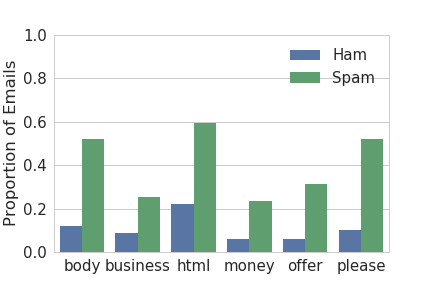
\includegraphics{training_conditional_proportions.png}
\caption{training conditional proportions}
\end{figure}

    \begin{Verbatim}[commandchars=\\\{\}]
{\color{incolor}In [{\color{incolor}9}]:} \PY{n}{train}\PY{o}{.}\PY{n}{head}\PY{p}{(}\PY{p}{)}
\end{Verbatim}


\begin{Verbatim}[commandchars=\\\{\}]
{\color{outcolor}Out[{\color{outcolor}9}]:}         id                                            subject  \textbackslash{}
        7657  7657             Subject: Patch to enable/disable log\textbackslash{}n   
        6911  6911        Subject: When an engineer flaps his wings\textbackslash{}n   
        6074  6074  Subject: Re: [Razor-users] razor plugins for m{\ldots}   
        4376  4376  Subject: NYTimes.com Article: Stop Those Press{\ldots}   
        5766  5766  Subject: What's facing FBI's new CIO? (Tech Up{\ldots}   
        
                                                          email  spam  
        7657  while i was playing with the past issues, it a{\ldots}     0  
        6911  url: http://diveintomark.org/archives/2002/10/{\ldots}     0  
        6074  no, please post a link!\textbackslash{}n \textbackslash{}n fox\textbackslash{}n ----- origi{\ldots}     0  
        4376  this article from nytimes.com \textbackslash{}n has been sent{\ldots}     0  
        5766  <html>\textbackslash{}n <head>\textbackslash{}n <title>tech update today</ti{\ldots}     0  
\end{Verbatim}
            
    \begin{Verbatim}[commandchars=\\\{\}]
{\color{incolor}In [{\color{incolor}117}]:} \PY{c+c1}{\PYZsh{} YOUR CODE HERE}
          \PY{n}{temp} \PY{o}{=} \PY{n}{train}\PY{o}{.}\PY{n}{reset\PYZus{}index}\PY{p}{(}\PY{p}{)}
          \PY{n}{words} \PY{o}{=} \PY{p}{[}\PY{l+s+s1}{\PYZsq{}}\PY{l+s+s1}{receive}\PY{l+s+s1}{\PYZsq{}}\PY{p}{,} \PY{l+s+s1}{\PYZsq{}}\PY{l+s+s1}{email}\PY{l+s+s1}{\PYZsq{}}\PY{p}{,} \PY{l+s+s1}{\PYZsq{}}\PY{l+s+s1}{contact}\PY{l+s+s1}{\PYZsq{}}\PY{p}{,} \PY{l+s+s1}{\PYZsq{}}\PY{l+s+s1}{click}\PY{l+s+s1}{\PYZsq{}}\PY{p}{,} \PY{l+s+s1}{\PYZsq{}}\PY{l+s+s1}{invest}\PY{l+s+s1}{\PYZsq{}}\PY{p}{,} \PY{l+s+s1}{\PYZsq{}}\PY{l+s+s1}{send}\PY{l+s+s1}{\PYZsq{}}\PY{p}{]}
          \PY{n}{df} \PY{o}{=} \PY{n}{pd}\PY{o}{.}\PY{n}{DataFrame}\PY{p}{(}\PY{n}{words\PYZus{}in\PYZus{}texts}\PY{p}{(}\PY{n}{words}\PY{p}{,} \PY{n}{temp}\PY{p}{[}\PY{l+s+s1}{\PYZsq{}}\PY{l+s+s1}{email}\PY{l+s+s1}{\PYZsq{}}\PY{p}{]}\PY{p}{)}\PY{p}{,} \PY{n}{columns}\PY{o}{=}\PY{n}{words}\PY{p}{)}
          \PY{n}{df}\PY{p}{[}\PY{l+s+s1}{\PYZsq{}}\PY{l+s+s1}{spam}\PY{l+s+s1}{\PYZsq{}}\PY{p}{]} \PY{o}{=} \PY{n}{temp}\PY{p}{[}\PY{l+s+s1}{\PYZsq{}}\PY{l+s+s1}{spam}\PY{l+s+s1}{\PYZsq{}}\PY{p}{]}
          \PY{n}{df} \PY{o}{=} \PY{n}{df}\PY{o}{.}\PY{n}{melt}\PY{p}{(}\PY{n}{id\PYZus{}vars} \PY{o}{=} \PY{l+s+s1}{\PYZsq{}}\PY{l+s+s1}{spam}\PY{l+s+s1}{\PYZsq{}}\PY{p}{)}
          
          \PY{n}{sns}\PY{o}{.}\PY{n}{barplot}\PY{p}{(}\PY{n}{x} \PY{o}{=} \PY{n}{df}\PY{p}{[}\PY{l+s+s1}{\PYZsq{}}\PY{l+s+s1}{variable}\PY{l+s+s1}{\PYZsq{}}\PY{p}{]}\PY{p}{,} \PY{n}{y} \PY{o}{=} \PY{n}{df}\PY{p}{[}\PY{l+s+s1}{\PYZsq{}}\PY{l+s+s1}{value}\PY{l+s+s1}{\PYZsq{}}\PY{p}{]}\PY{p}{,} \PY{n}{hue} \PY{o}{=} \PY{n}{df}\PY{p}{[}\PY{l+s+s1}{\PYZsq{}}\PY{l+s+s1}{spam}\PY{l+s+s1}{\PYZsq{}}\PY{p}{]}\PY{o}{.}\PY{n}{replace}\PY{p}{(}\PY{p}{[}\PY{l+m+mi}{0}\PY{p}{,} \PY{l+m+mi}{1}\PY{p}{]}\PY{p}{,} \PY{p}{[}\PY{l+s+s1}{\PYZsq{}}\PY{l+s+s1}{Ham}\PY{l+s+s1}{\PYZsq{}}\PY{p}{,} \PY{l+s+s1}{\PYZsq{}}\PY{l+s+s1}{Spam}\PY{l+s+s1}{\PYZsq{}}\PY{p}{]}\PY{p}{)}\PY{p}{,}  \PY{n}{ci}\PY{o}{=}\PY{k+kc}{None}\PY{p}{)}
          \PY{n}{plt}\PY{o}{.}\PY{n}{ylim}\PY{p}{(}\PY{l+m+mi}{0}\PY{p}{,} \PY{l+m+mi}{1}\PY{p}{)}
          \PY{n}{plt}\PY{o}{.}\PY{n}{ylabel}\PY{p}{(}\PY{l+s+s1}{\PYZsq{}}\PY{l+s+s1}{Proportion of Emails}\PY{l+s+s1}{\PYZsq{}}\PY{p}{)}
          \PY{n}{plt}\PY{o}{.}\PY{n}{legend}\PY{p}{(}\PY{p}{)}
          \PY{c+c1}{\PYZsh{}raise NotImplementedError()}
\end{Verbatim}


\begin{Verbatim}[commandchars=\\\{\}]
{\color{outcolor}Out[{\color{outcolor}117}]:} <matplotlib.legend.Legend at 0x7f0c98784978>
\end{Verbatim}
            
    \begin{center}
    \adjustimage{max size={0.9\linewidth}{0.9\paperheight}}{output_22_1.png}
    \end{center}
    { \hspace*{\fill} \\}
    
    \section{Question 3b}\label{question-3b}

When the feature is binary, it makes sense (as in the previous question)
to compare the proportion of 1s in the two classes of email. Otherwise,
if the feature can take on many values, it makes sense to compare the
distribution under spam to the distribution under ham. Create a
\emph{class conditional density plot} like the one below (which was
created using \texttt{sns.distplot}), comparing the distribution of a
feature among all spam emails to the distribution of the same feature
among all ham emails. \textbf{You may use the Fraction of Uppercase
Letters or create your own feature.}

\begin{figure}
\centering
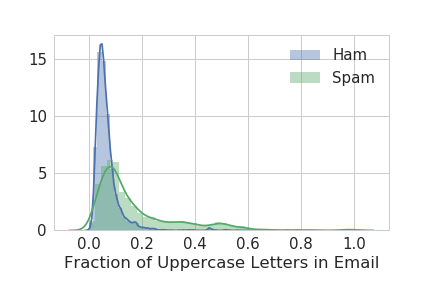
\includegraphics{training_conditional_densities2.png}
\caption{training conditional densities}
\end{figure}

    \begin{Verbatim}[commandchars=\\\{\}]
{\color{incolor}In [{\color{incolor}118}]:} \PY{c+c1}{\PYZsh{} YOUR CODE HERE}
          \PY{n}{temp} \PY{o}{=} \PY{n}{pd}\PY{o}{.}\PY{n}{read\PYZus{}csv}\PY{p}{(}\PY{l+s+s1}{\PYZsq{}}\PY{l+s+s1}{data/train.csv}\PY{l+s+s1}{\PYZsq{}}\PY{p}{)}
          \PY{p}{[}\PY{n}{train\PYZus{}temp}\PY{p}{,} \PY{n}{test\PYZus{}temp}\PY{p}{]} \PY{o}{=} \PY{n}{train\PYZus{}test\PYZus{}split}\PY{p}{(}\PY{n}{temp}\PY{p}{,} \PY{n}{test\PYZus{}size}\PY{o}{=}\PY{l+m+mf}{0.1}\PY{p}{,} \PY{n}{random\PYZus{}state}\PY{o}{=}\PY{l+m+mi}{42}\PY{p}{)}
          \PY{n}{train\PYZus{}temp}\PY{p}{[}\PY{l+s+s1}{\PYZsq{}}\PY{l+s+s1}{percentage}\PY{l+s+s1}{\PYZsq{}}\PY{p}{]} \PY{o}{=} \PY{n}{train\PYZus{}temp}\PY{p}{[}\PY{l+s+s1}{\PYZsq{}}\PY{l+s+s1}{email}\PY{l+s+s1}{\PYZsq{}}\PY{p}{]}\PY{o}{.}\PY{n}{str}\PY{o}{.}\PY{n}{findall}\PY{p}{(}\PY{l+s+s1}{\PYZsq{}}\PY{l+s+s1}{[A\PYZhy{}Z]}\PY{l+s+s1}{\PYZsq{}}\PY{p}{)}\PY{o}{.}\PY{n}{str}\PY{o}{.}\PY{n}{len}\PY{p}{(}\PY{p}{)} \PY{o}{/} \PY{n}{train\PYZus{}temp}\PY{p}{[}\PY{l+s+s1}{\PYZsq{}}\PY{l+s+s1}{email}\PY{l+s+s1}{\PYZsq{}}\PY{p}{]}\PY{o}{.}\PY{n}{str}\PY{o}{.}\PY{n}{findall}\PY{p}{(}\PY{l+s+s1}{\PYZsq{}}\PY{l+s+s1}{[a\PYZhy{}zA\PYZhy{}Z]}\PY{l+s+s1}{\PYZsq{}}\PY{p}{)}\PY{o}{.}\PY{n}{str}\PY{o}{.}\PY{n}{len}\PY{p}{(}\PY{p}{)}
          \PY{n}{sns}\PY{o}{.}\PY{n}{distplot}\PY{p}{(}\PY{n}{train\PYZus{}temp}\PY{p}{[}\PY{n}{train\PYZus{}temp}\PY{p}{[}\PY{l+s+s1}{\PYZsq{}}\PY{l+s+s1}{spam}\PY{l+s+s1}{\PYZsq{}}\PY{p}{]}\PY{o}{==}\PY{l+m+mi}{0}\PY{p}{]}\PY{p}{[}\PY{l+s+s1}{\PYZsq{}}\PY{l+s+s1}{percentage}\PY{l+s+s1}{\PYZsq{}}\PY{p}{]}\PY{p}{,} \PY{n}{label}\PY{o}{=}\PY{l+s+s1}{\PYZsq{}}\PY{l+s+s1}{Ham}\PY{l+s+s1}{\PYZsq{}}\PY{p}{)}
          \PY{n}{sns}\PY{o}{.}\PY{n}{distplot}\PY{p}{(}\PY{n}{train\PYZus{}temp}\PY{p}{[}\PY{n}{train\PYZus{}temp}\PY{p}{[}\PY{l+s+s1}{\PYZsq{}}\PY{l+s+s1}{spam}\PY{l+s+s1}{\PYZsq{}}\PY{p}{]}\PY{o}{==}\PY{l+m+mi}{1}\PY{p}{]}\PY{p}{[}\PY{l+s+s1}{\PYZsq{}}\PY{l+s+s1}{percentage}\PY{l+s+s1}{\PYZsq{}}\PY{p}{]}\PY{p}{,} \PY{n}{label}\PY{o}{=}\PY{l+s+s1}{\PYZsq{}}\PY{l+s+s1}{Spam}\PY{l+s+s1}{\PYZsq{}}\PY{p}{)}
          \PY{n}{plt}\PY{o}{.}\PY{n}{xlabel}\PY{p}{(}\PY{l+s+s1}{\PYZsq{}}\PY{l+s+s1}{Fraction of Uppercase Letters in Email}\PY{l+s+s1}{\PYZsq{}}\PY{p}{)}
          \PY{n}{plt}\PY{o}{.}\PY{n}{legend}\PY{p}{(}\PY{p}{)}
          \PY{c+c1}{\PYZsh{}raise NotImplementedError()}
\end{Verbatim}


    \begin{Verbatim}[commandchars=\\\{\}]
/srv/conda/envs/data100/lib/python3.6/site-packages/ipykernel\_launcher.py:4: SettingWithCopyWarning: 
A value is trying to be set on a copy of a slice from a DataFrame.
Try using .loc[row\_indexer,col\_indexer] = value instead

See the caveats in the documentation: http://pandas.pydata.org/pandas-docs/stable/indexing.html\#indexing-view-versus-copy
  after removing the cwd from sys.path.

    \end{Verbatim}

\begin{Verbatim}[commandchars=\\\{\}]
{\color{outcolor}Out[{\color{outcolor}118}]:} <matplotlib.legend.Legend at 0x7f0c9a8c9f98>
\end{Verbatim}
            
    \begin{center}
    \adjustimage{max size={0.9\linewidth}{0.9\paperheight}}{output_24_2.png}
    \end{center}
    { \hspace*{\fill} \\}
    
    \section{Basic Classification}\label{basic-classification}

Notice that the output of
\texttt{words\_in\_texts(words,\ train{[}\textquotesingle{}email\textquotesingle{}{]})}
is a numeric matrix containing features for each email. This means we
can use it directly to train a classifier!

    \section{Question 4}\label{question-4}

We've given you 5 words that might be useful as features to distinguish
spam/ham emails. Use these words as well as the \texttt{train} DataFrame
to create two NumPy arrays: \texttt{Phi\_train} and \texttt{Y\_train}.

\texttt{Phi\_train} should be a matrix of 0s and 1s created by using
your \texttt{words\_in\_texts} function on all the emails in the
training set.

\texttt{Y\_train} should be a vector of the correct labels for each
email in the training set.

    \begin{Verbatim}[commandchars=\\\{\}]
{\color{incolor}In [{\color{incolor}21}]:} \PY{n}{some\PYZus{}words} \PY{o}{=} \PY{p}{[}\PY{l+s+s1}{\PYZsq{}}\PY{l+s+s1}{drug}\PY{l+s+s1}{\PYZsq{}}\PY{p}{,} \PY{l+s+s1}{\PYZsq{}}\PY{l+s+s1}{bank}\PY{l+s+s1}{\PYZsq{}}\PY{p}{,} \PY{l+s+s1}{\PYZsq{}}\PY{l+s+s1}{prescription}\PY{l+s+s1}{\PYZsq{}}\PY{p}{,} \PY{l+s+s1}{\PYZsq{}}\PY{l+s+s1}{memo}\PY{l+s+s1}{\PYZsq{}}\PY{p}{,} \PY{l+s+s1}{\PYZsq{}}\PY{l+s+s1}{private}\PY{l+s+s1}{\PYZsq{}}\PY{p}{]}
         
         \PY{n}{Phi\PYZus{}train} \PY{o}{=} \PY{n}{words\PYZus{}in\PYZus{}texts}\PY{p}{(}\PY{n}{some\PYZus{}words}\PY{p}{,} \PY{n}{train}\PY{p}{[}\PY{l+s+s1}{\PYZsq{}}\PY{l+s+s1}{email}\PY{l+s+s1}{\PYZsq{}}\PY{p}{]}\PY{p}{)}
         \PY{n}{Y\PYZus{}train} \PY{o}{=} \PY{n}{train}\PY{p}{[}\PY{l+s+s1}{\PYZsq{}}\PY{l+s+s1}{spam}\PY{l+s+s1}{\PYZsq{}}\PY{p}{]}
         
         \PY{c+c1}{\PYZsh{} YOUR CODE HERE}
         \PY{c+c1}{\PYZsh{}raise NotImplementedError()}
         
         \PY{n}{Phi\PYZus{}train}\PY{p}{[}\PY{p}{:}\PY{l+m+mi}{5}\PY{p}{]}\PY{p}{,} \PY{n}{Y\PYZus{}train}\PY{p}{[}\PY{p}{:}\PY{l+m+mi}{5}\PY{p}{]}
\end{Verbatim}


\begin{Verbatim}[commandchars=\\\{\}]
{\color{outcolor}Out[{\color{outcolor}21}]:} (array([[0, 0, 0, 0, 0],
                 [0, 0, 0, 0, 0],
                 [0, 0, 0, 0, 0],
                 [0, 0, 0, 0, 0],
                 [0, 0, 0, 1, 0]]), 7657    0
          6911    0
          6074    0
          4376    0
          5766    0
          Name: spam, dtype: int64)
\end{Verbatim}
            
    \begin{Verbatim}[commandchars=\\\{\}]
{\color{incolor}In [{\color{incolor}22}]:} \PY{k}{assert} \PY{n}{np}\PY{o}{.}\PY{n}{all}\PY{p}{(}\PY{n}{np}\PY{o}{.}\PY{n}{unique}\PY{p}{(}\PY{n}{Phi\PYZus{}train}\PY{p}{)} \PY{o}{==} \PY{n}{np}\PY{o}{.}\PY{n}{array}\PY{p}{(}\PY{p}{[}\PY{l+m+mi}{0}\PY{p}{,} \PY{l+m+mi}{1}\PY{p}{]}\PY{p}{)}\PY{p}{)}
         \PY{k}{assert} \PY{n}{np}\PY{o}{.}\PY{n}{all}\PY{p}{(}\PY{n}{np}\PY{o}{.}\PY{n}{unique}\PY{p}{(}\PY{n}{Y\PYZus{}train}\PY{p}{)} \PY{o}{==} \PY{n}{np}\PY{o}{.}\PY{n}{array}\PY{p}{(}\PY{p}{[}\PY{l+m+mi}{0}\PY{p}{,} \PY{l+m+mi}{1}\PY{p}{]}\PY{p}{)}\PY{p}{)}
         \PY{k}{assert} \PY{n}{Phi\PYZus{}train}\PY{o}{.}\PY{n}{shape}\PY{p}{[}\PY{l+m+mi}{0}\PY{p}{]} \PY{o}{==} \PY{n}{Y\PYZus{}train}\PY{o}{.}\PY{n}{shape}\PY{p}{[}\PY{l+m+mi}{0}\PY{p}{]}
         \PY{k}{assert} \PY{n}{Phi\PYZus{}train}\PY{o}{.}\PY{n}{shape}\PY{p}{[}\PY{l+m+mi}{1}\PY{p}{]} \PY{o}{==} \PY{n+nb}{len}\PY{p}{(}\PY{n}{some\PYZus{}words}\PY{p}{)}
\end{Verbatim}


    \section{Question 5}\label{question-5}

Now we have matrices we can give to scikit-learn! Using the
\href{http://scikit-learn.org/stable/modules/generated/sklearn.linear_model.LogisticRegression.html}{\texttt{LogisticRegression}}
classifier, train a logistic regression model using \texttt{Phi\_train}
and \texttt{Y\_train}. Then, output the accuracy of the model (on the
training data) in the cell below. You should get an accuracy of around
0.75.

    \begin{Verbatim}[commandchars=\\\{\}]
{\color{incolor}In [{\color{incolor}23}]:} \PY{k+kn}{from} \PY{n+nn}{sklearn}\PY{n+nn}{.}\PY{n+nn}{linear\PYZus{}model} \PY{k}{import} \PY{n}{LogisticRegression} \PY{k}{as} \PY{n}{lm}
         \PY{n}{model} \PY{o}{=} \PY{n}{lm}\PY{p}{(}\PY{p}{)}
         \PY{n}{model}\PY{o}{.}\PY{n}{fit}\PY{p}{(}\PY{n}{Phi\PYZus{}train}\PY{p}{,} \PY{n}{Y\PYZus{}train}\PY{p}{)}
         \PY{c+c1}{\PYZsh{}print(model.predict(Phi\PYZus{}train))}
         \PY{n}{predict} \PY{o}{=} \PY{n}{model}\PY{o}{.}\PY{n}{predict}\PY{p}{(}\PY{n}{Phi\PYZus{}train}\PY{p}{)}
         \PY{n}{training\PYZus{}accuracy} \PY{o}{=} \PY{n}{model}\PY{o}{.}\PY{n}{score}\PY{p}{(}\PY{n}{Phi\PYZus{}train}\PY{p}{,} \PY{n}{Y\PYZus{}train}\PY{p}{)}
         
         \PY{n}{training\PYZus{}accuracy}
         \PY{c+c1}{\PYZsh{} YOUR CODE HERE}
         \PY{c+c1}{\PYZsh{}raise NotImplementedError()}
\end{Verbatim}


\begin{Verbatim}[commandchars=\\\{\}]
{\color{outcolor}Out[{\color{outcolor}23}]:} 0.75762012511646482
\end{Verbatim}
            
    \begin{Verbatim}[commandchars=\\\{\}]
{\color{incolor}In [{\color{incolor}24}]:} \PY{k}{assert} \PY{n}{training\PYZus{}accuracy} \PY{o}{\PYZgt{}} \PY{l+m+mf}{0.72}
\end{Verbatim}


    \section{Question 6}\label{question-6}

That doesn't seem too shabby! But the classifier you made above isn't as
good as this might lead us to believe. First, we are evaluating on the
training set, which may lead to a misleading accuracy measure,
especially if we used the training set to identify discriminative
features. In future parts of this analysis, it will be safer to hold out
some of our data for model validation and comparison.

Presumably, our classifier will be used for \textbf{filtering}, i.e.
preventing messages labelled \texttt{spam} from reaching someone's
inbox. Since we are trying There are two kinds of errors we can make: -
False positive (FP): a ham email gets flagged as spam and filtered out
of the inbox. - False negative (FN): a spam email gets mislabelled as
ham and ends up in the inbox.

These definitions depend both on the true labels and the predicted
labels. False positives and false negatives may be of differing
importance, leading us to consider more ways of evaluating a classifier,
in addition to overall accuracy:

\textbf{Precision} measures the proportion
\(\frac{\text{TP}}{\text{TP} + \text{FP}}\) of emails flagged as spam
that are actually spam.

\textbf{Recall} measures the proportion
\(\frac{\text{TP}}{\text{TP} + \text{FN}}\) of spam emails that were
correctly flagged as spam.

\textbf{False-alarm rate} measures the proportion
\(\frac{\text{FP}}{\text{FP} + \text{TN}}\) of ham emails that were
incorrectly flagged as spam.

The following image might help:

Note that a true positive (TP) is a spam email that is classified as
spam, and a true negative (TN) is a ham email that is classified as ham.
Answer the following questions in the cells below:

\begin{itemize}
\item
  \begin{enumerate}
  \def\labelenumi{(\alph{enumi})}
  \tightlist
  \item
    Suppose we have a classifier that just predicts 0 (ham) for every
    email. How many false positives are there? How many false negatives
    are there? Provide specific numbers using the training data from
    Question 4.
  \end{enumerate}
\item
  \begin{enumerate}
  \def\labelenumi{(\alph{enumi})}
  \setcounter{enumi}{1}
  \tightlist
  \item
    Suppose we have a classifier that just predicts 0 (ham) for every
    email. What is its accuracy on the training set? What is its recall
    on the training set?
  \end{enumerate}
\item
  \begin{enumerate}
  \def\labelenumi{(\alph{enumi})}
  \setcounter{enumi}{2}
  \tightlist
  \item
    What are the precision, recall, and false-alarm rate of the logistic
    regression classifier in Question 5? Are there more false positives
    or false negatives?
  \end{enumerate}
\item
  \begin{enumerate}
  \def\labelenumi{(\alph{enumi})}
  \setcounter{enumi}{3}
  \tightlist
  \item
    Our logistic regression classifier got 75.6\% prediction accuracy
    (number of correct predictions / total). How does this compare with
    predicting 0 for every email?
  \end{enumerate}
\item
  \begin{enumerate}
  \def\labelenumi{(\alph{enumi})}
  \setcounter{enumi}{4}
  \tightlist
  \item
    Given the word features we gave you above, name one reason this
    classifier is performing poorly.
  \end{enumerate}
\item
  \begin{enumerate}
  \def\labelenumi{(\alph{enumi})}
  \setcounter{enumi}{5}
  \tightlist
  \item
    Which of these two classifiers would you prefer for a spam filter
    and why? (N.B. there is no "right answer" here but be thoughtful in
    your reasoning).
  \end{enumerate}
\end{itemize}

    \begin{Verbatim}[commandchars=\\\{\}]
{\color{incolor}In [{\color{incolor}25}]:} \PY{c+c1}{\PYZsh{} provide number of FP and FN, respectively,}
         \PY{c+c1}{\PYZsh{} for a classifier that always predicts 0 (never predicts positive...)}
         \PY{n}{zero\PYZus{}predictor\PYZus{}fp} \PY{o}{=} \PY{l+m+mi}{0}
         \PY{n}{zero\PYZus{}predictor\PYZus{}fn} \PY{o}{=} \PY{n+nb}{len}\PY{p}{(}\PY{p}{[}\PY{n}{i} \PY{k}{for} \PY{n}{i} \PY{o+ow}{in} \PY{n}{Y\PYZus{}train} \PY{k}{if} \PY{n}{i} \PY{o}{==} \PY{l+m+mi}{1}\PY{p}{]}\PY{p}{)}
         
         \PY{n}{zero\PYZus{}predictor\PYZus{}fn}
         \PY{c+c1}{\PYZsh{} YOUR CODE HERE}
         \PY{c+c1}{\PYZsh{}raise NotImplementedError()}
\end{Verbatim}


\begin{Verbatim}[commandchars=\\\{\}]
{\color{outcolor}Out[{\color{outcolor}25}]:} 1918
\end{Verbatim}
            
    \begin{Verbatim}[commandchars=\\\{\}]
{\color{incolor}In [{\color{incolor}26}]:} \PY{c+c1}{\PYZsh{} This is a cell with just a comment but don\PYZsq{}t delete me if you want to get credit.}
\end{Verbatim}


    \begin{Verbatim}[commandchars=\\\{\}]
{\color{incolor}In [{\color{incolor}27}]:} \PY{c+c1}{\PYZsh{} provide training accuracy \PYZam{} recall, respectively,}
         \PY{c+c1}{\PYZsh{} for a classifier that always predicts 0}
         \PY{n}{zero\PYZus{}predictor\PYZus{}acc} \PY{o}{=} \PY{n+nb}{len}\PY{p}{(}\PY{p}{[}\PY{n}{i} \PY{k}{for} \PY{n}{i} \PY{o+ow}{in} \PY{n}{Y\PYZus{}train} \PY{k}{if} \PY{n}{i} \PY{o}{==} \PY{l+m+mi}{0}\PY{p}{]}\PY{p}{)}\PY{o}{/}\PY{n+nb}{len}\PY{p}{(}\PY{n}{Y\PYZus{}train}\PY{p}{)}
         \PY{n}{zero\PYZus{}predictor\PYZus{}recall} \PY{o}{=} \PY{l+m+mi}{0}
         
         \PY{n}{zero\PYZus{}predictor\PYZus{}acc}
         \PY{c+c1}{\PYZsh{}len(train)}
         \PY{c+c1}{\PYZsh{} YOUR CODE HERE}
         \PY{c+c1}{\PYZsh{}raise NotImplementedError()}
\end{Verbatim}


\begin{Verbatim}[commandchars=\\\{\}]
{\color{outcolor}Out[{\color{outcolor}27}]:} 0.7447091707706642
\end{Verbatim}
            
    \begin{Verbatim}[commandchars=\\\{\}]
{\color{incolor}In [{\color{incolor}28}]:} \PY{c+c1}{\PYZsh{} This is a cell with just a comment but don\PYZsq{}t delete me if you want to get credit.}
\end{Verbatim}


    \begin{Verbatim}[commandchars=\\\{\}]
{\color{incolor}In [{\color{incolor}29}]:} \PY{c+c1}{\PYZsh{} provide training accuracy \PYZam{} recall, respectively,}
         \PY{c+c1}{\PYZsh{} for logistic regression classifier from question 5}
         \PY{n}{predict} \PY{o}{=} \PY{n}{model}\PY{o}{.}\PY{n}{predict}\PY{p}{(}\PY{n}{Phi\PYZus{}train}\PY{p}{)}
         \PY{n}{actual} \PY{o}{=} \PY{n}{np}\PY{o}{.}\PY{n}{array}\PY{p}{(}\PY{n}{Y\PYZus{}train}\PY{p}{)}
         \PY{n}{true\PYZus{}pos} \PY{o}{=} \PY{n+nb}{len}\PY{p}{(}\PY{p}{[}\PY{n}{i} \PY{k}{for} \PY{n}{i} \PY{o+ow}{in} \PY{n+nb}{range}\PY{p}{(}\PY{n+nb}{len}\PY{p}{(}\PY{n}{predict}\PY{p}{)}\PY{p}{)} \PY{k}{if} \PY{n}{predict}\PY{p}{[}\PY{n}{i}\PY{p}{]} \PY{o}{==} \PY{l+m+mi}{1} \PY{o+ow}{and} \PY{n}{actual}\PY{p}{[}\PY{n}{i}\PY{p}{]} \PY{o}{==} \PY{l+m+mi}{1}\PY{p}{]}\PY{p}{)}
         \PY{n}{false\PYZus{}pos} \PY{o}{=} \PY{n+nb}{len}\PY{p}{(}\PY{p}{[}\PY{n}{i} \PY{k}{for} \PY{n}{i} \PY{o+ow}{in} \PY{n+nb}{range}\PY{p}{(}\PY{n+nb}{len}\PY{p}{(}\PY{n}{predict}\PY{p}{)}\PY{p}{)} \PY{k}{if} \PY{n}{predict}\PY{p}{[}\PY{n}{i}\PY{p}{]} \PY{o}{==} \PY{l+m+mi}{1} \PY{o+ow}{and} \PY{n}{actual}\PY{p}{[}\PY{n}{i}\PY{p}{]} \PY{o}{==} \PY{l+m+mi}{0}\PY{p}{]}\PY{p}{)}
         \PY{n}{false\PYZus{}neg} \PY{o}{=} \PY{n+nb}{len}\PY{p}{(}\PY{p}{[}\PY{n}{i} \PY{k}{for} \PY{n}{i} \PY{o+ow}{in} \PY{n+nb}{range}\PY{p}{(}\PY{n+nb}{len}\PY{p}{(}\PY{n}{predict}\PY{p}{)}\PY{p}{)} \PY{k}{if} \PY{n}{predict}\PY{p}{[}\PY{n}{i}\PY{p}{]} \PY{o}{==} \PY{l+m+mi}{0} \PY{o+ow}{and} \PY{n}{actual}\PY{p}{[}\PY{n}{i}\PY{p}{]} \PY{o}{==} \PY{l+m+mi}{1}\PY{p}{]}\PY{p}{)}
         \PY{n}{true\PYZus{}neg} \PY{o}{=} \PY{n+nb}{len}\PY{p}{(}\PY{p}{[}\PY{n}{i} \PY{k}{for} \PY{n}{i} \PY{o+ow}{in} \PY{n+nb}{range}\PY{p}{(}\PY{n+nb}{len}\PY{p}{(}\PY{n}{predict}\PY{p}{)}\PY{p}{)} \PY{k}{if} \PY{n}{predict}\PY{p}{[}\PY{n}{i}\PY{p}{]} \PY{o}{==} \PY{l+m+mi}{0} \PY{o+ow}{and} \PY{n}{actual}\PY{p}{[}\PY{n}{i}\PY{p}{]} \PY{o}{==} \PY{l+m+mi}{0}\PY{p}{]}\PY{p}{)}
         
         \PY{n}{logistic\PYZus{}predictor\PYZus{}precision} \PY{o}{=} \PY{n}{true\PYZus{}pos}\PY{o}{/}\PY{p}{(}\PY{n}{true\PYZus{}pos} \PY{o}{+} \PY{n}{false\PYZus{}pos}\PY{p}{)}
         \PY{n}{logistic\PYZus{}predictor\PYZus{}recall} \PY{o}{=} \PY{n}{true\PYZus{}pos}\PY{o}{/}\PY{p}{(}\PY{n}{true\PYZus{}pos} \PY{o}{+} \PY{n}{false\PYZus{}neg}\PY{p}{)}
         \PY{n}{logistic\PYZus{}predictor\PYZus{}far} \PY{o}{=} \PY{n}{false\PYZus{}pos} \PY{o}{/} \PY{p}{(}\PY{n}{false\PYZus{}pos} \PY{o}{+} \PY{n}{true\PYZus{}neg}\PY{p}{)}
         
         \PY{n+nb}{print}\PY{p}{(}\PY{n}{logistic\PYZus{}predictor\PYZus{}precision}\PY{p}{)}
         \PY{n+nb}{print}\PY{p}{(}\PY{n}{logistic\PYZus{}predictor\PYZus{}recall}\PY{p}{)}
         \PY{n+nb}{print}\PY{p}{(}\PY{n}{logistic\PYZus{}predictor\PYZus{}far}\PY{p}{)}
         \PY{c+c1}{\PYZsh{} YOUR CODE HERE}
         \PY{c+c1}{\PYZsh{}raise NotImplementedError()}
\end{Verbatim}


    \begin{Verbatim}[commandchars=\\\{\}]
0.6422287390029325
0.11418143899895725
0.021805183199285077

    \end{Verbatim}

    \begin{Verbatim}[commandchars=\\\{\}]
{\color{incolor}In [{\color{incolor}30}]:} \PY{n+nb}{print}\PY{p}{(}\PY{n}{false\PYZus{}pos}\PY{p}{)}
         \PY{n+nb}{print}\PY{p}{(}\PY{n}{false\PYZus{}neg}\PY{p}{)}
\end{Verbatim}


    \begin{Verbatim}[commandchars=\\\{\}]
122
1699

    \end{Verbatim}

    \begin{Verbatim}[commandchars=\\\{\}]
{\color{incolor}In [{\color{incolor}31}]:} \PY{c+c1}{\PYZsh{} This is a cell with just a comment but don\PYZsq{}t delete me if you want to get credit.}
\end{Verbatim}


    \begin{enumerate}
\def\labelenumi{(\alph{enumi})}
\item
  There are 0 false positives and 1918 false negatives.
\item
  The classifier's accuracy on the training set is roughly 74.5\%. Its
  recall is 0\%.
\item
  For the logistical regression classifier, the precision was about
  64.2\%, the recall was about 11.4\%, and the false-alarm rate was
  about 2.2\%. There were more false negatives than false positives
  (1699 false negatives and 122 false positives).
\item
  Our logistical regression classifier performed marginally better than
  the zero classifier, with roughly 75.6\% accuracy compared to the zero
  classifier's 74.5\% accuracy.
\item
  The logistical regression classifier is performing poorly because we
  only used 5 words as features when training and fitting our model, so
  we're most likely underfitting. We need more features to improve the
  accuracy of our model.
\item
  I'd prefer the zero classifier, since I'd rather not filter out any
  spam emails than accidentally filter out a ham email. Since the
  logistical regression classifier does not have a very high prediction
  accuracy, it could erroneously mark a ham email as spam and filter out
  that ham email, which may have important content. I'd rather not run
  that risk and just receive both ham and spam emails in my inbox so no
  important information is lost.
\end{enumerate}

    \section{Part II - Moving Forward}\label{part-ii---moving-forward}

With this in mind, it is now your task to make the spam filter more
accurate. In order to get full credit on the accuracy part of this
assignment, you must get at least \textbf{88\%} accuracy on the
evaluation set. To see your accuracy on the evaluation set, you will use
your classifier to predict every email in the \texttt{evaluation}
DataFrame and upload your predictions to Kaggle.

To prevent you from fitting to the evaluation set, you may only upload
predictions to Kaggle twice per day. This means you should start early
and rely on your \textbf{test data} to estimate your Kaggle scores.

Here are some ideas for improving your model:

\begin{enumerate}
\def\labelenumi{\arabic{enumi}.}
\tightlist
\item
  Finding better features based on the email text. Some example features
  are:

  \begin{enumerate}
  \def\labelenumii{\arabic{enumii}.}
  \tightlist
  \item
    Number of characters in the subject / body
  \item
    Number of words in the subject / body
  \item
    Use of punctuation (e.g., how many '!' were there?)
  \item
    Number / percentage of capital letters
  \item
    Whether the email is a reply to an earlier email or a forwarded
    email
  \end{enumerate}
\item
  Finding better words to use as features. Which words are the best at
  distinguishing emails? This requires digging into the email text
  itself.
\item
  Better data processing. For example, many emails contain HTML as well
  as text. You can consider extracting out the text from the HTML to
  help you find better words. Or, you can match HTML tags themselves, or
  even some combination of the two.
\item
  Model selection. You can adjust parameters of your model (e.g. the
  regularization parameter) to achieve higher accuracy. Recall that you
  should use cross-validation to do feature and model selection
  properly! Otherwise, you will likely overfit to your training data.
\end{enumerate}

You may use whatever method you prefer in order to create features.
However, \textbf{you are only allowed to train logistic regression
models and their regularized forms}. This means no random forest,
k-nearest-neighbors, neural nets, etc.

We will not give you a code skeleton to do this, so feel free to create
as many cells as you need in order to tackle this task. However,
answering questions 7, 8, and 9 should help guide you.

\begin{center}\rule{0.5\linewidth}{\linethickness}\end{center}

\textbf{Note:} \emph{You should use the \textbf{test data} to evaluate
your model and get a better sense of how it will perform on the Kaggle
evaluation.}

\begin{center}\rule{0.5\linewidth}{\linethickness}\end{center}

    \begin{Verbatim}[commandchars=\\\{\}]
{\color{incolor}In [{\color{incolor}138}]:} \PY{o}{!}pip install WordCloud
          \PY{k+kn}{import} \PY{n+nn}{collections}
          \PY{k+kn}{from} \PY{n+nn}{wordcloud} \PY{k}{import} \PY{n}{WordCloud}\PY{p}{,} \PY{n}{STOPWORDS}
          \PY{o}{\PYZpc{}}\PY{k}{matplotlib} inline
          \PY{k+kn}{from} \PY{n+nn}{sklearn}\PY{n+nn}{.}\PY{n+nn}{feature\PYZus{}extraction}\PY{n+nn}{.}\PY{n+nn}{text} \PY{k}{import} \PY{n}{CountVectorizer}
\end{Verbatim}


    \begin{Verbatim}[commandchars=\\\{\}]
Requirement already satisfied: WordCloud in /srv/conda/envs/data100/lib/python3.6/site-packages
Requirement already satisfied: pillow in /srv/conda/envs/data100/lib/python3.6/site-packages (from WordCloud)
Requirement already satisfied: numpy>=1.6.1 in /srv/conda/envs/data100/lib/python3.6/site-packages (from WordCloud)
Requirement already satisfied: matplotlib in /srv/conda/envs/data100/lib/python3.6/site-packages (from WordCloud)
Requirement already satisfied: six>=1.10 in /srv/conda/envs/data100/lib/python3.6/site-packages (from matplotlib->WordCloud)
Requirement already satisfied: python-dateutil>=2.0 in /srv/conda/envs/data100/lib/python3.6/site-packages (from matplotlib->WordCloud)
Requirement already satisfied: pytz in /srv/conda/envs/data100/lib/python3.6/site-packages (from matplotlib->WordCloud)
Requirement already satisfied: cycler>=0.10 in /srv/conda/envs/data100/lib/python3.6/site-packages (from matplotlib->WordCloud)
Requirement already satisfied: pyparsing!=2.0.4,!=2.1.2,!=2.1.6,>=2.0.1 in /srv/conda/envs/data100/lib/python3.6/site-packages (from matplotlib->WordCloud)
\textcolor{ansi-yellow}{You are using pip version 9.0.1, however version 10.0.1 is available.
You should consider upgrading via the 'pip install --upgrade pip' command.}

    \end{Verbatim}

    \begin{Verbatim}[commandchars=\\\{\}]
{\color{incolor}In [{\color{incolor}139}]:} \PY{n}{spam\PYZus{}data} \PY{o}{=} \PY{n}{train}\PY{p}{[}\PY{n}{train}\PY{p}{[}\PY{l+s+s1}{\PYZsq{}}\PY{l+s+s1}{spam}\PY{l+s+s1}{\PYZsq{}}\PY{p}{]} \PY{o}{==} \PY{l+m+mi}{1}\PY{p}{]}
          \PY{n}{spam\PYZus{}text} \PY{o}{=} \PY{n}{spam\PYZus{}data}\PY{o}{.}\PY{n}{email}\PY{o}{.}\PY{n}{str}\PY{o}{.}\PY{n}{cat}\PY{p}{(}\PY{n}{sep} \PY{o}{=} \PY{l+s+s1}{\PYZsq{}}\PY{l+s+s1}{ }\PY{l+s+s1}{\PYZsq{}}\PY{p}{)}
          
          \PY{n}{ham\PYZus{}data} \PY{o}{=} \PY{n}{train}\PY{p}{[}\PY{n}{train}\PY{p}{[}\PY{l+s+s1}{\PYZsq{}}\PY{l+s+s1}{spam}\PY{l+s+s1}{\PYZsq{}}\PY{p}{]} \PY{o}{==} \PY{l+m+mi}{0}\PY{p}{]}
          \PY{n}{ham\PYZus{}text} \PY{o}{=} \PY{n}{ham\PYZus{}data}\PY{o}{.}\PY{n}{email}\PY{o}{.}\PY{n}{str}\PY{o}{.}\PY{n}{cat}\PY{p}{(}\PY{n}{sep} \PY{o}{=} \PY{l+s+s1}{\PYZsq{}}\PY{l+s+s1}{ }\PY{l+s+s1}{\PYZsq{}}\PY{p}{)}
          
          \PY{k+kn}{import} \PY{n+nn}{re} 
          \PY{n}{spam\PYZus{}text} \PY{o}{=} \PY{n}{re}\PY{o}{.}\PY{n}{sub}\PY{p}{(}\PY{l+s+s1}{\PYZsq{}}\PY{l+s+s1}{\PYZlt{}[\PYZca{}\PYZlt{}]+?\PYZgt{}}\PY{l+s+s1}{\PYZsq{}}\PY{p}{,} \PY{l+s+s1}{\PYZsq{}}\PY{l+s+s1}{\PYZsq{}}\PY{p}{,} \PY{n}{spam\PYZus{}text}\PY{p}{)}
          \PY{n}{ham\PYZus{}text} \PY{o}{=} \PY{n}{re}\PY{o}{.}\PY{n}{sub}\PY{p}{(}\PY{l+s+s1}{\PYZsq{}}\PY{l+s+s1}{\PYZlt{}[\PYZca{}\PYZlt{}]+?\PYZgt{}}\PY{l+s+s1}{\PYZsq{}}\PY{p}{,} \PY{l+s+s1}{\PYZsq{}}\PY{l+s+s1}{\PYZsq{}}\PY{p}{,} \PY{n}{ham\PYZus{}text}\PY{p}{)}
\end{Verbatim}


    \begin{Verbatim}[commandchars=\\\{\}]
{\color{incolor}In [{\color{incolor}140}]:} \PY{c+c1}{\PYZsh{} stopwords = set(STOPWORDS)}
          \PY{c+c1}{\PYZsh{} spam\PYZus{}wordcount = \PYZob{}\PYZcb{}}
          
          \PY{c+c1}{\PYZsh{} for word in spam\PYZus{}text.lower().split():}
          \PY{c+c1}{\PYZsh{}     word = word.replace(\PYZdq{}.\PYZdq{},\PYZdq{}\PYZdq{})}
          \PY{c+c1}{\PYZsh{}     word = word.replace(\PYZdq{},\PYZdq{},\PYZdq{}\PYZdq{})}
          \PY{c+c1}{\PYZsh{}     word = word.replace(\PYZdq{}:\PYZdq{},\PYZdq{}\PYZdq{})}
          \PY{c+c1}{\PYZsh{}     word = word.replace(\PYZdq{}\PYZbs{}\PYZdq{}\PYZdq{},\PYZdq{}\PYZdq{})}
          \PY{c+c1}{\PYZsh{}     word = word.replace(\PYZdq{}!\PYZdq{},\PYZdq{}\PYZdq{})}
          \PY{c+c1}{\PYZsh{}     word = word.replace(\PYZdq{}“\PYZdq{},\PYZdq{}\PYZdq{})}
          \PY{c+c1}{\PYZsh{}     word = word.replace(\PYZdq{}‘\PYZdq{},\PYZdq{}\PYZdq{})}
          \PY{c+c1}{\PYZsh{}     word = word.replace(\PYZdq{}*\PYZdq{},\PYZdq{}\PYZdq{})}
          \PY{c+c1}{\PYZsh{}     if word not in stopwords:}
          \PY{c+c1}{\PYZsh{}         if word not in spam\PYZus{}wordcount:}
          \PY{c+c1}{\PYZsh{}             spam\PYZus{}wordcount[word] = 1}
          \PY{c+c1}{\PYZsh{}         else:}
          \PY{c+c1}{\PYZsh{}             spam\PYZus{}wordcount[word] += 1}
          \PY{c+c1}{\PYZsh{} \PYZsh{} Print most common words}
          \PY{c+c1}{\PYZsh{} n\PYZus{}print = int(input(\PYZdq{}How many most common words to print: \PYZdq{}))}
          \PY{c+c1}{\PYZsh{} word\PYZus{}counter = collections.Counter(spam\PYZus{}wordcount)}
          \PY{c+c1}{\PYZsh{} for word, count in word\PYZus{}counter.most\PYZus{}common(n\PYZus{}print):}
          \PY{c+c1}{\PYZsh{}     print(word, \PYZdq{}: \PYZdq{}, count)}
\end{Verbatim}


    \begin{Verbatim}[commandchars=\\\{\}]
{\color{incolor}In [{\color{incolor}141}]:} \PY{c+c1}{\PYZsh{} ham\PYZus{}wordcount = \PYZob{}\PYZcb{}}
          
          \PY{c+c1}{\PYZsh{} for word in ham\PYZus{}text.lower().split():}
          \PY{c+c1}{\PYZsh{}     word = word.replace(\PYZdq{}.\PYZdq{},\PYZdq{}\PYZdq{})}
          \PY{c+c1}{\PYZsh{}     word = word.replace(\PYZdq{},\PYZdq{},\PYZdq{}\PYZdq{})}
          \PY{c+c1}{\PYZsh{}     word = word.replace(\PYZdq{}:\PYZdq{},\PYZdq{}\PYZdq{})}
          \PY{c+c1}{\PYZsh{}     word = word.replace(\PYZdq{}\PYZbs{}\PYZdq{}\PYZdq{},\PYZdq{}\PYZdq{})}
          \PY{c+c1}{\PYZsh{}     word = word.replace(\PYZdq{}!\PYZdq{},\PYZdq{}\PYZdq{})}
          \PY{c+c1}{\PYZsh{}     word = word.replace(\PYZdq{}“\PYZdq{},\PYZdq{}\PYZdq{})}
          \PY{c+c1}{\PYZsh{}     word = word.replace(\PYZdq{}‘\PYZdq{},\PYZdq{}\PYZdq{})}
          \PY{c+c1}{\PYZsh{}     word = word.replace(\PYZdq{}*\PYZdq{},\PYZdq{}\PYZdq{})}
          \PY{c+c1}{\PYZsh{}     if word not in stopwords:}
          \PY{c+c1}{\PYZsh{}         if word not in ham\PYZus{}wordcount:}
          \PY{c+c1}{\PYZsh{}             ham\PYZus{}wordcount[word] = 1}
          \PY{c+c1}{\PYZsh{}         else:}
          \PY{c+c1}{\PYZsh{}             ham\PYZus{}wordcount[word] += 1}
          \PY{c+c1}{\PYZsh{} \PYZsh{} Print most common word}
          \PY{c+c1}{\PYZsh{} n\PYZus{}print = int(input(\PYZdq{}How many most common words to print: \PYZdq{}))}
          \PY{c+c1}{\PYZsh{} word\PYZus{}counter = collections.Counter(ham\PYZus{}wordcount)}
          \PY{c+c1}{\PYZsh{} for word, count in word\PYZus{}counter.most\PYZus{}common(n\PYZus{}print):}
          \PY{c+c1}{\PYZsh{}     print(word, \PYZdq{}: \PYZdq{}, count)}
\end{Verbatim}


    \begin{Verbatim}[commandchars=\\\{\}]
{\color{incolor}In [{\color{incolor}142}]:} \PY{c+c1}{\PYZsh{} for word in word\PYZus{}features:}
          \PY{c+c1}{\PYZsh{}     print(word + \PYZsq{}:\PYZsq{})}
          \PY{c+c1}{\PYZsh{}     print(\PYZsq{}ham \PYZhy{} \PYZsq{}+str(ham\PYZus{}wordcount[word]))}
          \PY{c+c1}{\PYZsh{}     print(\PYZsq{}spam \PYZhy{} \PYZsq{}+str(spam\PYZus{}wordcount[word]))}
          \PY{c+c1}{\PYZsh{}     print(\PYZsq{}\PYZsq{})}
\end{Verbatim}


    \begin{Verbatim}[commandchars=\\\{\}]
{\color{incolor}In [{\color{incolor}143}]:} \PY{c+c1}{\PYZsh{} word\PYZus{}features = [\PYZsq{}will\PYZsq{}, \PYZsq{}email\PYZsq{}, \PYZsq{}free\PYZsq{}, \PYZsq{}click\PYZsq{}, \PYZsq{}please\PYZsq{}, \PYZsq{}money\PYZsq{}, \PYZsq{}business\PYZsq{}, \PYZsq{}list\PYZsq{}, \PYZsq{}one\PYZsq{},\PYZsq{}information\PYZsq{},}
          \PY{c+c1}{\PYZsh{}                   \PYZsq{}receive\PYZsq{}, \PYZsq{}e\PYZhy{}mail\PYZsq{}, \PYZsq{}people\PYZsq{}, \PYZsq{}address\PYZsq{}, \PYZsq{}name\PYZsq{}, \PYZsq{}time\PYZsq{}, \PYZsq{}new\PYZsq{}, \PYZsq{}send\PYZsq{}, \PYZsq{}make\PYZsq{}, \PYZsq{}order\PYZsq{}, \PYZsq{}report\PYZsq{},}
          \PY{c+c1}{\PYZsh{}                  \PYZsq{}message\PYZsq{}, \PYZsq{}want\PYZsq{}, \PYZsq{}home\PYZsq{},\PYZsq{}removed\PYZsq{}, \PYZsq{}may\PYZsq{}, \PYZsq{}program\PYZsq{}, \PYZsq{}de\PYZsq{}, \PYZsq{}company\PYZsq{},}
          \PY{c+c1}{\PYZsh{}                  \PYZsq{}government\PYZsq{}, \PYZsq{}form\PYZsq{}, \PYZsq{}offer\PYZsq{}, \PYZsq{}credit\PYZsq{}, \PYZsq{}best\PYZsq{}, \PYZsq{}life\PYZsq{}, \PYZsq{}use\PYZsq{}, \PYZsq{}need\PYZsq{}, \PYZsq{}million\PYZsq{}, \PYZsq{}content\PYZhy{}type\PYZsq{},}
          \PY{c+c1}{\PYZsh{}                  \PYZsq{}site\PYZsq{}, \PYZsq{}go\PYZsq{}, \PYZsq{}help\PYZsq{}, \PYZsq{}software\PYZsq{}, \PYZsq{}call\PYZsq{}, \PYZsq{}work\PYZsq{}, \PYZsq{}today\PYZsq{}, \PYZsq{}wish\PYZsq{}, \PYZsq{}phone\PYZsq{}, \PYZsq{}web\PYZsq{},\PYZsq{}first\PYZsq{}, \PYZsq{}remove\PYZsq{},}
          \PY{c+c1}{\PYZsh{}                  \PYZsq{}marketing\PYZsq{}, \PYZsq{}mail\PYZsq{}, \PYZsq{}service\PYZsq{}, \PYZsq{}within\PYZsq{}, \PYZsq{}grants\PYZsq{}, \PYZsq{}state\PYZsq{}, \PYZsq{}reply\PYZsq{}, \PYZsq{}sent\PYZsq{}, \PYZsq{}day\PYZsq{}, \PYZsq{}every\PYZsq{}, \PYZsq{}insurance\PYZsq{},}
          \PY{c+c1}{\PYZsh{}                  \PYZsq{}online\PYZsq{}, \PYZsq{}take\PYZsq{}, \PYZsq{}per\PYZsq{}, \PYZsq{}special\PYZsq{}, \PYZsq{}price\PYZsq{}, \PYZsq{}much\PYZsq{}, \PYZsq{}see\PYZsq{}, \PYZsq{}received\PYZsq{}, \PYZsq{}year\PYZsq{}, \PYZsq{}made\PYZsq{},}
          \PY{c+c1}{\PYZsh{}                  \PYZsq{}contact\PYZsq{}, \PYZsq{}even\PYZsq{}, \PYZsq{}number\PYZsq{}, \PYZsq{}addresses\PYZsq{}, \PYZsq{}available\PYZsq{}, \PYZsq{}cash\PYZsq{}, \PYZsq{}orders\PYZsq{}, \PYZsq{}know\PYZsq{}, \PYZsq{}future\PYZsq{}]}
          
          \PY{c+c1}{\PYZsh{} \PYZsh{}word\PYZus{}features = list(unique\PYZus{}words)}
          \PY{c+c1}{\PYZsh{} Phi\PYZus{}train = words\PYZus{}in\PYZus{}texts(word\PYZus{}features, train[\PYZsq{}email\PYZsq{}])}
          \PY{c+c1}{\PYZsh{} Y\PYZus{}train = train[\PYZsq{}spam\PYZsq{}]}
          
          \PY{c+c1}{\PYZsh{} Phi\PYZus{}test = words\PYZus{}in\PYZus{}texts(word\PYZus{}features, test[\PYZsq{}email\PYZsq{}])}
          \PY{c+c1}{\PYZsh{} Y\PYZus{}test = test[\PYZsq{}spam\PYZsq{}]}
          
          \PY{c+c1}{\PYZsh{} from sklearn.linear\PYZus{}model import LogisticRegression as lm}
          \PY{c+c1}{\PYZsh{} model = lm()}
          \PY{c+c1}{\PYZsh{} model.fit(Phi\PYZus{}train, Y\PYZus{}train)}
          \PY{c+c1}{\PYZsh{} training\PYZus{}accuracy = model.score(Phi\PYZus{}train, Y\PYZus{}train)}
          \PY{c+c1}{\PYZsh{} test\PYZus{}accuracy = model.score(Phi\PYZus{}test, Y\PYZus{}test)}
          
          \PY{c+c1}{\PYZsh{} print(\PYZsq{}Training Score: \PYZsq{} + str(training\PYZus{}accuracy))}
          \PY{c+c1}{\PYZsh{} print(\PYZsq{}Test Score: \PYZsq{} + str(test\PYZus{}accuracy))}
\end{Verbatim}


    \begin{Verbatim}[commandchars=\\\{\}]
{\color{incolor}In [{\color{incolor}144}]:} \PY{n}{vector} \PY{o}{=} \PY{n}{CountVectorizer}\PY{p}{(}\PY{p}{)}
          \PY{n}{Phi\PYZus{}train} \PY{o}{=} \PY{n}{vector}\PY{o}{.}\PY{n}{fit\PYZus{}transform}\PY{p}{(}\PY{n}{train}\PY{p}{[}\PY{l+s+s1}{\PYZsq{}}\PY{l+s+s1}{email}\PY{l+s+s1}{\PYZsq{}}\PY{p}{]}\PY{p}{)}
          \PY{n}{Phi\PYZus{}test} \PY{o}{=} \PY{n}{vector}\PY{o}{.}\PY{n}{transform}\PY{p}{(}\PY{n}{test}\PY{p}{[}\PY{l+s+s1}{\PYZsq{}}\PY{l+s+s1}{email}\PY{l+s+s1}{\PYZsq{}}\PY{p}{]}\PY{p}{)}
          \PY{n}{Y\PYZus{}train} \PY{o}{=} \PY{n}{train}\PY{p}{[}\PY{l+s+s1}{\PYZsq{}}\PY{l+s+s1}{spam}\PY{l+s+s1}{\PYZsq{}}\PY{p}{]}
          \PY{n}{Y\PYZus{}test} \PY{o}{=} \PY{n}{test}\PY{p}{[}\PY{l+s+s1}{\PYZsq{}}\PY{l+s+s1}{spam}\PY{l+s+s1}{\PYZsq{}}\PY{p}{]}
          
          \PY{n}{model} \PY{o}{=} \PY{n}{lm}\PY{p}{(}\PY{p}{)}
          \PY{n}{model}\PY{o}{.}\PY{n}{fit}\PY{p}{(}\PY{n}{Phi\PYZus{}train}\PY{p}{,} \PY{n}{Y\PYZus{}train}\PY{p}{)}
          \PY{n}{training\PYZus{}accuracy} \PY{o}{=} \PY{n}{model}\PY{o}{.}\PY{n}{score}\PY{p}{(}\PY{n}{Phi\PYZus{}train}\PY{p}{,} \PY{n}{Y\PYZus{}train}\PY{p}{)}
          \PY{n}{test\PYZus{}accuracy} \PY{o}{=} \PY{n}{model}\PY{o}{.}\PY{n}{score}\PY{p}{(}\PY{n}{Phi\PYZus{}test}\PY{p}{,} \PY{n}{Y\PYZus{}test}\PY{p}{)}
          
          \PY{n+nb}{print}\PY{p}{(}\PY{l+s+s1}{\PYZsq{}}\PY{l+s+s1}{Training Score: }\PY{l+s+s1}{\PYZsq{}} \PY{o}{+} \PY{n+nb}{str}\PY{p}{(}\PY{n}{training\PYZus{}accuracy}\PY{p}{)}\PY{p}{)}
          \PY{n+nb}{print}\PY{p}{(}\PY{l+s+s1}{\PYZsq{}}\PY{l+s+s1}{Test Score: }\PY{l+s+s1}{\PYZsq{}} \PY{o}{+} \PY{n+nb}{str}\PY{p}{(}\PY{n}{test\PYZus{}accuracy}\PY{p}{)}\PY{p}{)}
\end{Verbatim}


    \begin{Verbatim}[commandchars=\\\{\}]
Training Score: 0.999600692134
Test Score: 0.991616766467

    \end{Verbatim}

    \section{Question 7 (Feature/Model Selection
Process)}\label{question-7-featuremodel-selection-process}

In this following cell, describe the process of improving your model.
You should use at least 2-3 sentences each to address the follow
questions:

\begin{enumerate}
\def\labelenumi{\arabic{enumi}.}
\tightlist
\item
  How did you find better features for your model?
\item
  What did you try that worked / didn't work?
\item
  What was surprising in your search for good features?
\end{enumerate}

    \begin{enumerate}
\def\labelenumi{\arabic{enumi}.}
\item
  I found better features for my model by using the CountVectorizer
  class from Scikit Learn, which allowed me to convert the training data
  emails to a matrix of counts for each word. CountVectorizer has a
  fit\_transform() method, which I used to learn the vocabulary from the
  input training emails (the training email column), and then transform
  the email text into an encoded vector. The encoded vector consists of
  an integer count for the number of times each word appeared in the
  emails, and is a sparse matrix. I used this matrix as my Phi\_train
  (the features) and fit my model using Phi\_train and the true labels
  for training data (Y\_train), and got a very high training and testing
  accuracy (roughly 99\%).
\item
  The first feature extraction method I tried was simply taking the text
  of all spam emails, finding the counts of each word in the spam
  emails, and calling words\_in\_texts on a list of the 100 most common
  spam words to obtain my word features. I had a lot of html tags as my
  features, which wasn't very useful information, so then I removed html
  tags before finding the word counts and creating my word features. I
  then manually tested adding/removing some words from my features to
  see how it changed my training and testing accuracies, which actually
  helped me achieve about 92\% accuracy. However, the sklearn
  CountVectorizer class performed better with 99\% accuracy, so I
  ultimately discarded my initial approach of choosing the most common
  spam words.
\item
  I originally thought that using too many features would be overfitting
  to my training data, and my classifier wouldn't perform as well on my
  testing data with so many features. I was surprised to find that
  although using CountVectorizer without putting a limit on the maximum
  number of features returned a very, very large number of features, it
  performed much better than when I did limit the maximum number of
  features.
\end{enumerate}

    \section{Question 8 (EDA)}\label{question-8-eda}

In the two cells below, show a visualization that you used to select
features for your model. Include both

\begin{enumerate}
\def\labelenumi{\arabic{enumi}.}
\tightlist
\item
  A plot showing something meaningful about the data that helped you
  during feature / model selection.
\item
  2-3 sentences describing what you plotted and what its implications
  are for your features.
\end{enumerate}

Feel to create as many plots as you want in your process of feature
selection, but select one for the cells below.

\textbf{You should not show us a visualization just like in question 3.}
Specifically, don't show us a bar chart of proportions, or a
one-dimensional class conditional density plot. Any other plot is
acceptable, as long as it comes with thoughtful commentary. Here are
some ideas:

\begin{enumerate}
\def\labelenumi{\arabic{enumi}.}
\tightlist
\item
  Consider the correlation between multiple features (look up
  correlation plots and \texttt{sns.heatmap}).
\item
  Try to show redundancy in a group of features (e.g. \texttt{body} and
  \texttt{html} might co-occur relatively frequently, or you might be
  able to design a feature that captures all html tags and compare it to
  these).
\item
  Use a word-cloud or another visualization tool to characterize the
  most common spam words.
\item
  Visually depict whether spam emails tend to be wordier (in some sense)
  than ham emails.
\end{enumerate}

    \begin{Verbatim}[commandchars=\\\{\}]
{\color{incolor}In [{\color{incolor}146}]:} \PY{c+c1}{\PYZsh{} YOUR CODE HERE}
          \PY{c+c1}{\PYZsh{} I used a code snippet that I found on Stack Overflow to generate a word cloud, source link is below:}
          \PY{c+c1}{\PYZsh{} source: https://stackoverflow.com/questions/16645799/how\PYZhy{}to\PYZhy{}create\PYZhy{}a\PYZhy{}word\PYZhy{}cloud\PYZhy{}from\PYZhy{}a\PYZhy{}corpus\PYZhy{}in\PYZhy{}python?utm\PYZus{}medium=organic\PYZam{}utm\PYZus{}source=google\PYZus{}rich\PYZus{}qa\PYZam{}utm\PYZus{}campaign=google\PYZus{}rich\PYZus{}qa}
          \PY{n}{stopwords} \PY{o}{=} \PY{n+nb}{set}\PY{p}{(}\PY{n}{STOPWORDS}\PY{p}{)}
          
          \PY{k}{def} \PY{n+nf}{show\PYZus{}wordcloud}\PY{p}{(}\PY{n}{data}\PY{p}{,} \PY{n}{title} \PY{o}{=} \PY{l+s+s1}{\PYZsq{}}\PY{l+s+s1}{Most Common Spam Words}\PY{l+s+s1}{\PYZsq{}}\PY{p}{)}\PY{p}{:}
              \PY{n}{wordcloud} \PY{o}{=} \PY{n}{WordCloud}\PY{p}{(}
                  \PY{n}{background\PYZus{}color}\PY{o}{=}\PY{l+s+s1}{\PYZsq{}}\PY{l+s+s1}{white}\PY{l+s+s1}{\PYZsq{}}\PY{p}{,}
                  \PY{n}{stopwords}\PY{o}{=}\PY{n}{stopwords}\PY{p}{,}
                  \PY{n}{max\PYZus{}words}\PY{o}{=}\PY{l+m+mi}{200}\PY{p}{,}
                  \PY{n}{max\PYZus{}font\PYZus{}size}\PY{o}{=}\PY{l+m+mi}{50}\PY{p}{,} 
                  \PY{n}{scale}\PY{o}{=}\PY{l+m+mi}{3}\PY{p}{,}
                  \PY{n}{random\PYZus{}state}\PY{o}{=}\PY{l+m+mi}{1}
              \PY{p}{)}\PY{o}{.}\PY{n}{generate}\PY{p}{(}\PY{n+nb}{str}\PY{p}{(}\PY{n}{data}\PY{p}{)}\PY{p}{)}
          
              \PY{n}{fig} \PY{o}{=} \PY{n}{plt}\PY{o}{.}\PY{n}{figure}\PY{p}{(}\PY{l+m+mi}{1}\PY{p}{,} \PY{n}{figsize}\PY{o}{=}\PY{p}{(}\PY{l+m+mi}{12}\PY{p}{,} \PY{l+m+mi}{12}\PY{p}{)}\PY{p}{)}
              \PY{n}{plt}\PY{o}{.}\PY{n}{axis}\PY{p}{(}\PY{l+s+s1}{\PYZsq{}}\PY{l+s+s1}{off}\PY{l+s+s1}{\PYZsq{}}\PY{p}{)}
              \PY{k}{if} \PY{n}{title}\PY{p}{:} 
                  \PY{n}{fig}\PY{o}{.}\PY{n}{suptitle}\PY{p}{(}\PY{n}{title}\PY{p}{,} \PY{n}{fontsize}\PY{o}{=}\PY{l+m+mi}{20}\PY{p}{)}
                  \PY{n}{fig}\PY{o}{.}\PY{n}{subplots\PYZus{}adjust}\PY{p}{(}\PY{n}{top}\PY{o}{=}\PY{l+m+mf}{2.3}\PY{p}{)}
          
              \PY{n}{plt}\PY{o}{.}\PY{n}{imshow}\PY{p}{(}\PY{n}{wordcloud}\PY{p}{)}
              \PY{n}{plt}\PY{o}{.}\PY{n}{show}\PY{p}{(}\PY{p}{)}
          
          \PY{n}{show\PYZus{}wordcloud}\PY{p}{(}\PY{n}{spam\PYZus{}text}\PY{p}{)}
          \PY{c+c1}{\PYZsh{}show\PYZus{}wordcloud(ham\PYZus{}text)}
          \PY{c+c1}{\PYZsh{}raise NotImplementedError()}
\end{Verbatim}


    \begin{center}
    \adjustimage{max size={0.9\linewidth}{0.9\paperheight}}{output_52_0.png}
    \end{center}
    { \hspace*{\fill} \\}
    
    I plotted a wordcloud that displays the 200 most common words in spam
emails, with font size and different colors representing the frequencies
of each word. This was helpful for choosing words as features, since the
most common words would be more helpful as features in my classifier
than less common words. With my original feature extraction method, I
programmatically found the 100 most common spam words, manually added
some words in the wordcloud and removed some words not in the wordcloud,
and this helped improve my accuracy.

(The wordcoud was helpful for my original feature extraction method, but
later I used CountVectorizer to improve my classifier's accuracy and did
not manually choose features).

    \section{Question 9 (Making a Precision-Recall
Curve)}\label{question-9-making-a-precision-recall-curve}

We can trade off between precision and recall. In most cases we won't be
able to get both perfect precision (i.e. no false positives) and recall
(i.e. no false negatives), so we have to compromise. For example, in the
case of cancer screenings, false negatives are comparatively worse than
false positives --- a false negative means that a patient might not
discover a disease until it's too late to treat, while a false positive
means that a patient will probably have to take another screening.

Recall that logistic regression calculates the probability that an
example belongs to a certain class. Then, to classify an example we say
that an email is spam if our classifier gives it \(\ge 0.5\) probability
of being spam. However, \emph{we can adjust that cutoff}: we can say
that an email is spam only if our classifier gives it \(\ge 0.7\)
probability of being spam, for example. This is how we can trade off
false positives and false negatives.

The precision-recall curve shows this trade off for each possible cutoff
probability. In the cell below,
\href{http://scikit-learn.org/stable/auto_examples/model_selection/plot_precision_recall.html\#plot-the-precision-recall-curve}{plot
a precision-recall curve} for your final classifier (the one you use to
make predictions for Kaggle).

    \begin{Verbatim}[commandchars=\\\{\}]
{\color{incolor}In [{\color{incolor}147}]:} \PY{k+kn}{from} \PY{n+nn}{sklearn}\PY{n+nn}{.}\PY{n+nn}{metrics} \PY{k}{import} \PY{n}{precision\PYZus{}recall\PYZus{}curve}
          
          \PY{c+c1}{\PYZsh{} Note that you\PYZsq{}ll want to use the .predict\PYZus{}proba(...) method for your classifier}
          \PY{c+c1}{\PYZsh{} instead of .predict(...) so you get probabilities, not classes}
          \PY{n}{Y\PYZus{}test} \PY{o}{=} \PY{n}{test}\PY{p}{[}\PY{l+s+s1}{\PYZsq{}}\PY{l+s+s1}{spam}\PY{l+s+s1}{\PYZsq{}}\PY{p}{]}
          \PY{n}{y\PYZus{}score} \PY{o}{=} \PY{n}{model}\PY{o}{.}\PY{n}{predict\PYZus{}proba}\PY{p}{(}\PY{n}{Phi\PYZus{}test}\PY{p}{)}\PY{p}{[}\PY{p}{:}\PY{p}{,} \PY{l+m+mi}{1}\PY{p}{]}
          \PY{n}{precision}\PY{p}{,} \PY{n}{recall}\PY{p}{,} \PY{n}{\PYZus{}} \PY{o}{=} \PY{n}{precision\PYZus{}recall\PYZus{}curve}\PY{p}{(}\PY{n}{Y\PYZus{}test}\PY{p}{,} \PY{n}{y\PYZus{}score}\PY{p}{)}
          
          \PY{n}{plt}\PY{o}{.}\PY{n}{step}\PY{p}{(}\PY{n}{recall}\PY{p}{,} \PY{n}{precision}\PY{p}{,} \PY{n}{color}\PY{o}{=}\PY{l+s+s1}{\PYZsq{}}\PY{l+s+s1}{b}\PY{l+s+s1}{\PYZsq{}}\PY{p}{,} \PY{n}{alpha}\PY{o}{=}\PY{l+m+mf}{0.2}\PY{p}{,}
                   \PY{n}{where}\PY{o}{=}\PY{l+s+s1}{\PYZsq{}}\PY{l+s+s1}{post}\PY{l+s+s1}{\PYZsq{}}\PY{p}{)}
          \PY{n}{plt}\PY{o}{.}\PY{n}{fill\PYZus{}between}\PY{p}{(}\PY{n}{recall}\PY{p}{,} \PY{n}{precision}\PY{p}{,} \PY{n}{step}\PY{o}{=}\PY{l+s+s1}{\PYZsq{}}\PY{l+s+s1}{post}\PY{l+s+s1}{\PYZsq{}}\PY{p}{,} \PY{n}{alpha}\PY{o}{=}\PY{l+m+mf}{0.2}\PY{p}{,}
                           \PY{n}{color}\PY{o}{=}\PY{l+s+s1}{\PYZsq{}}\PY{l+s+s1}{b}\PY{l+s+s1}{\PYZsq{}}\PY{p}{)}
          
          \PY{n}{plt}\PY{o}{.}\PY{n}{xlabel}\PY{p}{(}\PY{l+s+s1}{\PYZsq{}}\PY{l+s+s1}{Recall}\PY{l+s+s1}{\PYZsq{}}\PY{p}{)}
          \PY{n}{plt}\PY{o}{.}\PY{n}{ylabel}\PY{p}{(}\PY{l+s+s1}{\PYZsq{}}\PY{l+s+s1}{Precision}\PY{l+s+s1}{\PYZsq{}}\PY{p}{)}
          \PY{n}{plt}\PY{o}{.}\PY{n}{ylim}\PY{p}{(}\PY{p}{[}\PY{l+m+mf}{0.0}\PY{p}{,} \PY{l+m+mf}{1.05}\PY{p}{]}\PY{p}{)}
          \PY{n}{plt}\PY{o}{.}\PY{n}{xlim}\PY{p}{(}\PY{p}{[}\PY{l+m+mf}{0.0}\PY{p}{,} \PY{l+m+mf}{1.0}\PY{p}{]}\PY{p}{)}
          \PY{n}{plt}\PY{o}{.}\PY{n}{title}\PY{p}{(}\PY{l+s+s1}{\PYZsq{}}\PY{l+s+s1}{2\PYZhy{}class Precision\PYZhy{}Recall curve}\PY{l+s+s1}{\PYZsq{}}\PY{p}{)}
          \PY{c+c1}{\PYZsh{} YOUR CODE HERE}
          \PY{c+c1}{\PYZsh{}raise NotImplementedError()}
\end{Verbatim}


\begin{Verbatim}[commandchars=\\\{\}]
{\color{outcolor}Out[{\color{outcolor}147}]:} Text(0.5,1,'2-class Precision-Recall curve')
\end{Verbatim}
            
    \begin{center}
    \adjustimage{max size={0.9\linewidth}{0.9\paperheight}}{output_55_1.png}
    \end{center}
    { \hspace*{\fill} \\}
    
    \section{Question 10: Submitting to
Kaggle}\label{question-10-submitting-to-kaggle}

The following code will write your predictions on the evaluation dataset
to a CSV, which you can submit to Kaggle. You may need to modify it to
suit your needs.

Save your predictions in a 1-dimensional array called
\texttt{evaluation\_predictions}. \emph{Even if you are not submitting
to Kaggle, please make sure you've saved your predictions to
\texttt{evaluation\_predictions} as this is how your grade for this part
will be determined.}

Remember that if you've performed transformations or featurization on
the training data, you must also perform the same transformations on the
evaluation data in order to make predictions. For example, if you've
created features for the words "drug" and "money" on the training data,
you must also extract the same features in order to use scikit-learn's
\texttt{.predict(...)} method.

You should submit your CSV files to
https://www.kaggle.com/t/39fae66747b14fd48fe0984f2e4f16ac

    \begin{Verbatim}[commandchars=\\\{\}]
{\color{incolor}In [{\color{incolor}94}]:} \PY{c+c1}{\PYZsh{} CHANGE ME (Currently making random predictions)}
         \PY{c+c1}{\PYZsh{} model = lm()}
         \PY{c+c1}{\PYZsh{} Phi\PYZus{}train = words\PYZus{}in\PYZus{}texts(word\PYZus{}features, train[\PYZsq{}email\PYZsq{}])}
         \PY{c+c1}{\PYZsh{} Y\PYZus{}train = train[\PYZsq{}spam\PYZsq{}]}
         \PY{c+c1}{\PYZsh{} model.fit(Phi\PYZus{}train, Y\PYZus{}train)}
         \PY{c+c1}{\PYZsh{} Phi\PYZus{}eval = words\PYZus{}in\PYZus{}texts(word\PYZus{}features, evaluation[\PYZsq{}email\PYZsq{}])}
         \PY{n}{Phi\PYZus{}eval} \PY{o}{=} \PY{n}{vector}\PY{o}{.}\PY{n}{transform}\PY{p}{(}\PY{n}{evaluation}\PY{p}{[}\PY{l+s+s1}{\PYZsq{}}\PY{l+s+s1}{email}\PY{l+s+s1}{\PYZsq{}}\PY{p}{]}\PY{p}{)}
         \PY{n}{evaluation\PYZus{}predictions} \PY{o}{=} \PY{n}{model}\PY{o}{.}\PY{n}{predict}\PY{p}{(}\PY{n}{Phi\PYZus{}eval}\PY{p}{)}
         \PY{n}{evaluation\PYZus{}predictions}
         \PY{c+c1}{\PYZsh{} YOUR CODE HERE}
         \PY{c+c1}{\PYZsh{}raise NotImplementedError()}
\end{Verbatim}


\begin{Verbatim}[commandchars=\\\{\}]
{\color{outcolor}Out[{\color{outcolor}94}]:} array([0, 1, 1, 0, 0, 0, 1, 0, 0, 0, 1, 0, 0, 0, 0, 0, 1, 0, 0, 0, 0, 1, 0,
                0, 0, 0, 0, 1, 1, 0, 0, 0, 0, 1, 0, 0, 0, 0, 0, 0, 0, 0, 0, 0, 0, 1,
                0, 0, 1, 0, 0, 0, 0, 0, 0, 0, 0, 0, 0, 1, 1, 0, 0, 1, 0, 0, 0, 1, 1,
                0, 0, 0, 0, 0, 0, 1, 0, 0, 0, 0, 0, 1, 0, 0, 0, 1, 1, 0, 0, 1, 0, 0,
                0, 0, 1, 0, 0, 1, 0, 1, 0, 0, 0, 0, 0, 0, 0, 0, 0, 0, 0, 0, 0, 0, 1,
                0, 1, 0, 1, 1, 0, 0, 0, 0, 0, 0, 0, 0, 0, 0, 0, 0, 0, 0, 0, 1, 0, 1,
                0, 0, 1, 0, 0, 0, 0, 0, 0, 0, 0, 0, 0, 0, 0, 0, 1, 0, 0, 0, 0, 0, 1,
                0, 1, 0, 0, 1, 0, 1, 0, 0, 0, 0, 0, 1, 0, 0, 0, 0, 0, 0, 1, 0, 0, 0,
                1, 0, 1, 0, 0, 0, 1, 0, 0, 0, 1, 0, 0, 1, 0, 0, 0, 0, 1, 0, 0, 0, 0,
                0, 0, 0, 0, 0, 0, 0, 1, 1, 0, 0, 0, 0, 0, 1, 0, 0, 1, 0, 0, 0, 0, 1,
                0, 1, 0, 0, 0, 0, 0, 0, 1, 0, 0, 0, 1, 1, 0, 0, 0, 0, 0, 1, 0, 0, 0,
                1, 0, 1, 0, 1, 0, 1, 1, 0, 1, 1, 0, 0, 0, 0, 0, 0, 0, 0, 0, 0, 0, 1,
                0, 0, 0, 0, 0, 0, 0, 0, 0, 0, 0, 1, 0, 1, 0, 0, 0, 0, 1, 0, 0, 1, 0,
                1, 1, 1, 0, 0, 0, 0, 0, 0, 1, 1, 0, 0, 0, 1, 1, 0, 0, 0, 0, 0, 0, 0,
                1, 0, 0, 0, 0, 0, 0, 0, 0, 1, 0, 0, 1, 0, 0, 0, 0, 1, 0, 0, 1, 0, 1,
                0, 1, 0, 0, 0, 1, 0, 0, 0, 0, 0, 0, 1, 1, 1, 0, 0, 0, 0, 1, 0, 0, 0,
                0, 1, 0, 1, 0, 0, 0, 1, 0, 0, 1, 1, 1, 0, 0, 0, 1, 0, 0, 1, 1, 0, 1,
                0, 1, 1, 0, 0, 1, 1, 0, 0, 0, 1, 1, 0, 0, 0, 0, 0, 1, 0, 0, 1, 0, 0,
                0, 1, 0, 0, 1, 1, 0, 0, 0, 0, 0, 1, 0, 0, 0, 0, 0, 1, 1, 0, 0, 1, 1,
                1, 0, 0, 1, 0, 1, 0, 0, 0, 0, 0, 0, 0, 0, 0, 1, 0, 0, 0, 0, 0, 1, 0,
                0, 0, 0, 0, 1, 0, 0, 0, 0, 0, 1, 0, 0, 0, 0, 0, 0, 1, 0, 0, 0, 1, 1,
                1, 1, 0, 0, 0, 0, 1, 0, 0, 0, 0, 1, 0, 0, 1, 0, 0, 0, 1, 0, 0, 1, 0,
                0, 0, 0, 1, 0, 0, 0, 0, 1, 0, 0, 0, 1, 0, 1, 1, 0, 0, 0, 0, 0, 0, 1,
                1, 0, 1, 1, 0, 0, 1, 1, 0, 0, 0, 0, 0, 0, 1, 0, 0, 0, 0, 0, 0, 0, 0,
                0, 0, 0, 0, 1, 0, 1, 1, 0, 0, 1, 0, 0, 0, 0, 1, 0, 0, 0, 0, 0, 0, 0,
                1, 0, 0, 0, 1, 0, 0, 0, 0, 0, 0, 0, 0, 0, 0, 0, 1, 0, 0, 0, 0, 1, 0,
                0, 0, 0, 1, 0, 0, 0, 0, 0, 0, 1, 0, 0, 0, 0, 1, 1, 0, 0, 0, 1, 0, 0,
                0, 1, 0, 0, 0, 0, 1, 0, 0, 0, 1, 1, 0, 0, 1, 0, 1, 0, 0, 0, 1, 1, 1,
                0, 1, 0, 0, 0, 0, 0, 0, 0, 0, 0, 0, 0, 1, 0, 0, 0, 0, 0, 0, 0, 0, 0,
                0, 0, 1, 0, 0, 0, 1, 0, 0, 1, 1, 0, 0, 0, 0, 0, 0, 1, 1, 1, 1, 0, 0,
                0, 0, 0, 0, 0, 1, 0, 0, 0, 0, 0, 0, 0, 0, 1, 0, 0, 1, 0, 0, 0, 0, 0,
                0, 1, 0, 0, 0, 1, 0, 0, 0, 0, 1, 1, 1, 0, 1, 1, 1, 0, 1, 0, 0, 0, 0,
                1, 0, 0, 0, 0, 0, 1, 1, 0, 0, 0, 0, 0, 0, 0, 0, 0, 1, 0, 0, 0, 0, 0,
                0, 0, 1, 0, 1, 0, 0, 0, 0, 0, 0, 0, 0, 0, 1, 1, 0, 0, 0, 0, 1, 1, 0,
                0, 0, 0, 1, 1, 0, 0, 0, 0, 0, 0, 0, 1, 0, 0, 0, 1, 0, 0, 1, 0, 0, 0,
                0, 1, 0, 0, 1, 0, 0, 0, 1, 0, 0, 1, 0, 0, 0, 0, 0, 0, 0, 0, 0, 0, 1,
                0, 1, 0, 0, 0, 0, 0, 1, 1, 0, 0, 0, 0, 0, 0, 0, 0, 1, 0, 0, 0, 0, 0,
                0, 1, 1, 0, 0, 0, 1, 0, 0, 0, 0, 0, 0, 0, 0, 0, 0, 0, 0, 0, 0, 1, 0,
                0, 0, 1, 1, 0, 0, 1, 0, 1, 1, 0, 0, 0, 0, 0, 1, 0, 0, 1, 0, 0, 1, 0,
                1, 0, 1, 0, 1, 0, 1, 0, 0, 0, 0, 0, 0, 0, 0, 0, 0, 0, 0, 0, 1, 0, 0,
                0, 1, 1, 0, 0, 0, 0, 1, 0, 1, 1, 0, 1, 0, 1, 0, 1, 0, 0, 0, 0, 0, 1,
                0, 0, 0, 1, 0, 0, 0, 1, 0, 1, 0, 0, 1, 0, 1, 1, 0, 0, 1, 0, 0, 0, 0,
                1, 0, 0, 0, 0, 0, 1, 0, 0, 1, 0, 1, 1, 0, 0, 0, 0, 0, 0, 0, 0, 0, 0,
                0, 1, 0, 0, 0, 0, 0, 0, 0, 0, 1])
\end{Verbatim}
            
    \begin{Verbatim}[commandchars=\\\{\}]
{\color{incolor}In [{\color{incolor}148}]:} \PY{c+c1}{\PYZsh{} must be ndarray of predictions}
          \PY{k}{assert} \PY{n+nb}{isinstance}\PY{p}{(}\PY{n}{evaluation\PYZus{}predictions}\PY{p}{,} \PY{n}{np}\PY{o}{.}\PY{n}{ndarray}\PY{p}{)} 
          
          \PY{c+c1}{\PYZsh{} must be binary labels (0 or 1) and not probabilities}
          \PY{k}{assert} \PY{n}{np}\PY{o}{.}\PY{n}{all}\PY{p}{(}\PY{p}{(}\PY{n}{evaluation\PYZus{}predictions} \PY{o}{==} \PY{l+m+mi}{0}\PY{p}{)} \PY{o}{|} \PY{p}{(}\PY{n}{evaluation\PYZus{}predictions} \PY{o}{==} \PY{l+m+mi}{1}\PY{p}{)}\PY{p}{)}
          
          \PY{c+c1}{\PYZsh{} must be the right number of predictions}
          \PY{k}{assert} \PY{n}{evaluation\PYZus{}predictions}\PY{o}{.}\PY{n}{shape} \PY{o}{==} \PY{p}{(}\PY{l+m+mi}{1000}\PY{p}{,} \PY{p}{)}
\end{Verbatim}


    \begin{Verbatim}[commandchars=\\\{\}]
{\color{incolor}In [{\color{incolor}96}]:} \PY{c+c1}{\PYZsh{} Please do not modify this cell}
\end{Verbatim}


    The following saves a file to submit to Kaggle.

    \begin{Verbatim}[commandchars=\\\{\}]
{\color{incolor}In [{\color{incolor}97}]:} \PY{k+kn}{from} \PY{n+nn}{datetime} \PY{k}{import} \PY{n}{datetime}
         
         \PY{c+c1}{\PYZsh{} Assuming that your predictions on the evaluation set are stored in a 1\PYZhy{}dimensional array called}
         \PY{c+c1}{\PYZsh{} evaluation\PYZus{}predictions. Feel free to modify this cell as long you create a CSV in the right format.}
         
         \PY{c+c1}{\PYZsh{} must be ndarray of predictions}
         \PY{k}{assert} \PY{n+nb}{isinstance}\PY{p}{(}\PY{n}{evaluation\PYZus{}predictions}\PY{p}{,} \PY{n}{np}\PY{o}{.}\PY{n}{ndarray}\PY{p}{)} 
         
         \PY{c+c1}{\PYZsh{} must be binary labels (0 or 1) and not probabilities}
         \PY{k}{assert} \PY{n}{np}\PY{o}{.}\PY{n}{all}\PY{p}{(}\PY{p}{(}\PY{n}{evaluation\PYZus{}predictions} \PY{o}{==} \PY{l+m+mi}{0}\PY{p}{)} \PY{o}{|} \PY{p}{(}\PY{n}{evaluation\PYZus{}predictions} \PY{o}{==} \PY{l+m+mi}{1}\PY{p}{)}\PY{p}{)}
         
         \PY{c+c1}{\PYZsh{} must be the right number of predictions}
         \PY{k}{assert} \PY{n}{evaluation\PYZus{}predictions}\PY{o}{.}\PY{n}{shape} \PY{o}{==} \PY{p}{(}\PY{l+m+mi}{1000}\PY{p}{,} \PY{p}{)}
         
         \PY{c+c1}{\PYZsh{} Construct and save the submission:}
         \PY{n}{submission\PYZus{}df} \PY{o}{=} \PY{n}{pd}\PY{o}{.}\PY{n}{DataFrame}\PY{p}{(}\PY{p}{\PYZob{}}
             \PY{l+s+s2}{\PYZdq{}}\PY{l+s+s2}{Id}\PY{l+s+s2}{\PYZdq{}}\PY{p}{:} \PY{n}{evaluation}\PY{p}{[}\PY{l+s+s1}{\PYZsq{}}\PY{l+s+s1}{id}\PY{l+s+s1}{\PYZsq{}}\PY{p}{]}\PY{p}{,} 
             \PY{l+s+s2}{\PYZdq{}}\PY{l+s+s2}{Class}\PY{l+s+s2}{\PYZdq{}}\PY{p}{:} \PY{n}{evaluation\PYZus{}predictions}\PY{p}{,}
         \PY{p}{\PYZcb{}}\PY{p}{,} \PY{n}{columns}\PY{o}{=}\PY{p}{[}\PY{l+s+s1}{\PYZsq{}}\PY{l+s+s1}{Id}\PY{l+s+s1}{\PYZsq{}}\PY{p}{,} \PY{l+s+s1}{\PYZsq{}}\PY{l+s+s1}{Class}\PY{l+s+s1}{\PYZsq{}}\PY{p}{]}\PY{p}{)}
         \PY{n}{timestamp} \PY{o}{=} \PY{n}{datetime}\PY{o}{.}\PY{n}{isoformat}\PY{p}{(}\PY{n}{datetime}\PY{o}{.}\PY{n}{now}\PY{p}{(}\PY{p}{)}\PY{p}{)}\PY{o}{.}\PY{n}{split}\PY{p}{(}\PY{l+s+s2}{\PYZdq{}}\PY{l+s+s2}{.}\PY{l+s+s2}{\PYZdq{}}\PY{p}{)}\PY{p}{[}\PY{l+m+mi}{0}\PY{p}{]}
         \PY{n}{submission\PYZus{}df}\PY{o}{.}\PY{n}{to\PYZus{}csv}\PY{p}{(}\PY{l+s+s2}{\PYZdq{}}\PY{l+s+s2}{submission\PYZus{}}\PY{l+s+si}{\PYZob{}\PYZcb{}}\PY{l+s+s2}{.csv}\PY{l+s+s2}{\PYZdq{}}\PY{o}{.}\PY{n}{format}\PY{p}{(}\PY{n}{timestamp}\PY{p}{)}\PY{p}{,} \PY{n}{index}\PY{o}{=}\PY{k+kc}{False}\PY{p}{)}
         
         \PY{n+nb}{print}\PY{p}{(}\PY{l+s+s1}{\PYZsq{}}\PY{l+s+s1}{Created a CSV file: }\PY{l+s+si}{\PYZob{}\PYZcb{}}\PY{l+s+s1}{.}\PY{l+s+s1}{\PYZsq{}}\PY{o}{.}\PY{n}{format}\PY{p}{(}\PY{l+s+s2}{\PYZdq{}}\PY{l+s+s2}{submission\PYZus{}}\PY{l+s+si}{\PYZob{}\PYZcb{}}\PY{l+s+s2}{.csv}\PY{l+s+s2}{\PYZdq{}}\PY{o}{.}\PY{n}{format}\PY{p}{(}\PY{n}{timestamp}\PY{p}{)}\PY{p}{)}\PY{p}{)}
         \PY{n+nb}{print}\PY{p}{(}\PY{l+s+s1}{\PYZsq{}}\PY{l+s+s1}{You may now upload this CSV file to Kaggle for scoring.}\PY{l+s+s1}{\PYZsq{}}\PY{p}{)}
\end{Verbatim}


    \begin{Verbatim}[commandchars=\\\{\}]
Created a CSV file: submission\_2018-04-30T19:43:07.csv.
You may now upload this CSV file to Kaggle for scoring.

    \end{Verbatim}


    % Add a bibliography block to the postdoc
    
    
    
    \end{document}
